\documentclass[11pt,a4paper]{article}

\usepackage{fontspec}
\setmainfont{NotoSansSC-Task1-Subset.ttf}[
  Path=fonts/,
  BoldFont=NotoSansSC-Task1-Subset.ttf,
  BoldFeatures={FakeBold=2},
  ItalicFont=NotoSansSC-Task1-Subset.ttf,
  ItalicFeatures={FakeSlant=0.18},
  BoldItalicFont=NotoSansSC-Task1-Subset.ttf,
  BoldItalicFeatures={FakeBold=2,FakeSlant=0.18}
]
\setsansfont{NotoSansSC-Task1-Subset.ttf}[Path=fonts/,BoldFont=NotoSansSC-Task1-Subset.ttf,BoldFeatures={FakeBold=2}]
\setmonofont{NotoSansSC-Task1-Subset.ttf}[Path=fonts/,Scale=MatchLowercase]
\XeTeXlinebreaklocale "zh"
\XeTeXlinebreakskip=0pt plus 1pt
\usepackage[a4paper,top=22mm,bottom=22mm,left=21mm,right=21mm,headheight=15pt]{geometry}
\usepackage{amsmath,amssymb}
\usepackage{graphicx}
\usepackage{booktabs}
\usepackage{tabularx}
\usepackage{longtable}
\usepackage{array}
\usepackage{multirow}
\usepackage{makecell}
\usepackage{threeparttable}
\usepackage{float}
\usepackage{caption}
\usepackage{subcaption}
\usepackage{pdflscape}
\usepackage{adjustbox}
\usepackage{enumitem}
\usepackage{xcolor}
\usepackage[most]{tcolorbox}
\usepackage{fancyhdr}
\usepackage{lastpage}
\usepackage{hyperref}
\usepackage[nameinlink,noabbrev]{cleveref}

\definecolor{DeepBlue}{HTML}{0B5A7A}
\definecolor{Teal}{HTML}{008B78}
\definecolor{Amber}{HTML}{D98300}
\definecolor{SoftBlue}{HTML}{EAF4F8}
\definecolor{SoftAmber}{HTML}{FFF4DE}
\definecolor{SoftRed}{HTML}{FDECEC}
\definecolor{Muted}{HTML}{555555}

\hypersetup{
  colorlinks=true,
  linkcolor=DeepBlue,
  citecolor=Teal,
  urlcolor=DeepBlue,
  pdftitle={原始 Frankenstein-v28 N-甲基化扩展 ProteinMPNN 的单体与复合物评估},
  pdfauthor={项目组（内部中文审阅稿）}
}
\urlstyle{tt}

\captionsetup{font=small,labelfont=bf,labelsep=quad}
\setlist{nosep,leftmargin=2em}
\setlength{\parindent}{2em}
\setlength{\parskip}{0.15em}
\setlength{\emergencystretch}{1em}
\renewcommand{\arraystretch}{1.18}
\newcolumntype{Y}{>{\raggedright\arraybackslash}X}
\newcolumntype{C}[1]{>{\centering\arraybackslash}p{#1}}
\newcolumntype{L}[1]{>{\raggedright\arraybackslash}p{#1}}
\newcommand{\seq}[1]{\texttt{#1}}
\newcommand{\NA}{\textemdash}
\newcommand{\angstrom}{\text{\AA}}
\newcommand{\taskone}{Task~1}
\newcommand{\checkpointsha}{\texttt{bab7b8a0\allowbreak{}10114fc5\allowbreak{}2c749fab\allowbreak{}1914d9d8\allowbreak{}ae561ddc\allowbreak{}a45d6d7a\allowbreak{}0fbec3f9\allowbreak{}f5ac5b2e}}
\newcommand{\checkpointshort}{\texttt{bab7b8a0\ldots f5ac5b2e}}

\renewcommand{\contentsname}{目录}
\renewcommand{\listfigurename}{图目录}
\renewcommand{\listtablename}{表目录}
\renewcommand{\figurename}{图}
\renewcommand{\tablename}{表}
\renewcommand{\refname}{参考文献}

\crefname{figure}{图}{图}
\crefname{table}{表}{表}
\crefname{section}{节}{节}
\crefname{appendix}{附录}{附录}

\pagestyle{fancy}
\fancyhf{}
\fancyhead[L]{原始 Frankenstein-v28：Task 1 中文论文稿}
\fancyhead[R]{\small 2026-08-21}
\fancyfoot[C]{第 \thepage\ 页，共 \pageref{LastPage} 页}
\renewcommand{\headrulewidth}{0.4pt}

\title{\bfseries\LARGE 原始 Frankenstein-v28 N-甲基化扩展 ProteinMPNN 的单体与复合物评估\\[0.45em]
\large Ser 来源修正、六个非 3AV 复合物的预设分析与 17 靶点探索性证据}
\author{项目组（作者与单位信息待补）}
\date{中文内部审阅稿 v1.0｜2026年8月21日}

\begin{document}

\begin{titlepage}
  \centering
  \vspace*{22mm}
  {\color{DeepBlue}\bfseries\LARGE 原始 Frankenstein-v28 N-甲基化扩展 ProteinMPNN 的单体与复合物评估\par}
  \vspace{4mm}
  {\Large Ser 来源修正、六个非 3AV 复合物的预设分析与 17 靶点探索性证据\par}
  \vspace{12mm}
  {\large 项目组（作者与单位信息待补）\par}
  \vspace{3mm}
  {\large 中文内部审阅稿 v1.0｜2026年8月21日\par}
  \vfill
  \begin{tcolorbox}[width=0.92\textwidth,colback=SoftBlue,colframe=DeepBlue,boxrule=0.8pt,arc=2mm]
    \textbf{冻结对象：}未经后续 V7/V8/V9 修改的原始 \path{frankenstein_v28.pt}。\\
    \textbf{SHA-256：}\checkpointsha\\
    \textbf{仓库基线：}\path{DCarchimonde/proteinmpnn-clean-v28@c9718e2a}（完整提交见源清单）。\\
    \textbf{稿件性质：}Task 1 的完整中文解释稿；所有可报告结果、不可报告指标、历史错误口径和数据缺口均在同一文档中列明。
  \end{tcolorbox}
  \vspace{6mm}
  {\small 本稿不把预测置信度称为能量，不把肽自对齐 RMSD 称为结合姿态，不把 oracle best-of-N 结果称为无偏生成性能。\par}
\end{titlepage}

\section*{摘要}
\addcontentsline{toc}{section}{摘要}

\textbf{目的：}对未经后续修改的原始 \path{frankenstein_v28.pt} 进行一次可追溯的回顾性评价，并把单体、六个非 3AV 复合物的预设主分析以及 17 靶点的探索性下游结果统一到同一篇中文稿件中。

\textbf{方法：}模型文件由 SHA-256 冻结。单体留出集含 151 个 Rosetta 理论结构、1505 个真实序列位点；751 个单体原始 PDB 全部标记为 Rosetta 理论模型，不存在可核验的“Baker 33 真结构”子集。来源审计发现旧标签中有 62 个 Ser 被错误标为 N-甲基化；在不改变模型权重与预测概率的前提下，将评价真值修正为 261 个阳性与 1244 个阴性。甲基化阈值预设为严格大于 0.6。复合物主分析仅纳入 1SFI、3P8F、3WNE、3ZGC、4K1E 和 4KEL，在温度 0.5 下保留至少一个已保存甲基化标记的序列。结构判定要求全复合物 CA 在一次全局对齐后，复合物全局 CA RMSD 与末链环肽的 best-forward 循环移位 CA RMSD 同时严格低于同一阈值。17 靶点 best85 结果因按天然序列恢复率进行 best-of-N 选择，仅作探索性支持。

\textbf{结果：}单体天然化氨基酸恢复率（RAA）为 16.08\%，完整扩展 token 恢复率为 14.88\%。修正标签后，已知天然序列甲基分类 AUC 为 0.900，在阈值 $>0.6$ 时 Accuracy、Precision、Recall 和 F1 分别为 86.18\%、64.02\%、46.36\% 和 53.78\%；端到端 AUC 为 0.908，对应四项指标为 89.10\%、88.80\%、42.53\% 和 57.51\%。端到端二分类甲基召回为 111/261（42.53\%），但同时恢复正确天然氨基酸身份和甲基状态的真实甲基残基仅 20/261（7.66\%）。六复合物在温度 0.5 下共有 544 条原始序列，476 条（87.50\%）满足甲基化保留门且全部匹配结构 RMSD。联合 RMSD $<3\,\angstrom$ 为 16/476（3.36\%，Wilson 95\% CI 2.08--5.39\%），$<5\,\angstrom$ 为 101/476（21.22\%，17.78--25.11\%）；以全部 544 条原始序列为分母，端到端产率分别为 2.94\% 和 18.57\%。17 靶点 best85 的肽受体框架 CA RMSD 均值/中位数为 29.93/40.06~\AA，而肽自对齐 CA RMSD 为 2.65/2.53~\AA；这表明内部形状与结合姿态必须分开解释。其平均结构多样性 $1-\mathrm{TM}$ 为 0.660；预测通透性、置信度与自然化 fixed-pose Rosetta 分数仅作为描述性证据。

\textbf{结论：}原始模型在单体甲基化位点排序上具有辨别力，但在阈值 0.6 下召回率中等，且基础序列恢复率较低。六复合物的严格端到端产率显示，主要瓶颈是环肽在同一复合物坐标系中的结合姿态，而非受体/全局对齐本身。当前证据支持把本结果作为模型能力边界与下一轮改进基线，而不支持宣称已实现高成功率结构设计。单体结构 RMSD、显式全原子甲基 RMSD、结合位点恢复、相对天然能量成功率与稳定性尚无可核验结果，未作填补。

\noindent\textbf{关键词：}N-甲基化环肽；ProteinMPNN；序列设计；甲基化分类；RMSD；端到端产率；数据来源审计

\begin{tcolorbox}[colback=SoftAmber,colframe=Amber,title=读者先看这三句话]
  \begin{enumerate}
    \item 正文单体指标使用“去 padding、Ser 来源修正、阈值严格 $>0.6$”口径；用户提供的两张旧终端截图只在附录进行错误复盘。
    \item 六复合物的 3.36\% 与 21.22\% 是通过甲基化保留门后的条件比例；真正从原始 544 条序列出发的产率是 2.94\% 与 18.57\%。
    \item best85 是利用天然序列恢复率选出的 oracle 代表，不是未知天然序列时可直接获得的部署性能。
  \end{enumerate}
\end{tcolorbox}


\clearpage
\tableofcontents
\clearpage
\listoffigures
\listoftables
\clearpage

\section{引言}

ProteinMPNN 以给定蛋白骨架为条件生成氨基酸序列，原始工作表明其能够处理单链与多链设计问题\cite{dauparas2022proteinmpnn}。本项目在此基础上增加了 N-甲基化表示：先预测天然氨基酸，再由与天然残基类别相对应的甲基化专家头给出位点置信度。因此，模型实际上同时面对两个相互耦合但不等价的问题：

\begin{enumerate}
  \item \textbf{基础序列问题：}给定结构，天然化后的氨基酸是否恢复正确；
  \item \textbf{甲基化问题：}在已知或模型预测的天然氨基酸条件下，该位点是否应标记为 N-甲基化；
  \item \textbf{结构问题：}生成序列形成的结构是否保持合理的内部构象，并处于正确的受体结合姿态。
\end{enumerate}

这三类问题不能用一个数字代替。较高的甲基分类 AUC 不等于较高的天然序列恢复率；较低的肽自对齐 RMSD 也不等于正确结合；结构预测文件中的 B-factor/pLDDT 代理值更不是物理能量。为了避免这些概念在先前零散汇报中互相混淆，本研究将所有可追溯证据按数据队列和评价定义重新组织。

本稿只完成 \taskone，研究对象严格冻结为原始 \path{frankenstein_v28.pt}。后续 V7、V8、V9 的训练、拼接或稳定性修复不属于本文结果。核心问题包括：

\begin{itemize}
  \item 原始模型在单体留出集上的 RAA、AUC、Accuracy、Precision、Recall 与 F1 到底是多少；
  \item 为什么先前截图出现 16.59\%、38.11\% 与 85.67\% 等值，以及它们能否用于论文；
  \item 在温度 0.5、甲基化置信度严格 $>0.6$ 的条件下，六个非 3AV 复合物从原始序列到联合 RMSD $<3$~\AA 或 $<5$~\AA 的真实产率是多少；
  \item 17 靶点的 best85 结构、置信度、多样性、通透性与 fixed-pose 能量能说明什么，又不能说明什么；
  \item 尚哥提出的全部指标中，哪些已经有合格证据，哪些仍未计算或在数学上不可定义。
\end{itemize}

论文的主张边界是保守且明确的：我们报告已经观测到的模型输出和结构计算结果，但不从预测分数外推实验透膜性、结合自由能或生物活性；不把缺失值填成零；不以选择后的代表样本替代完整生成分母。

\section{材料与方法}

\subsection{模型冻结与可追溯性}

全文只评价原始检查点 \path{frankenstein_v28.pt}，SHA-256 为 \checkpointsha。检查点包含 ProteinMPNN 风格的共享结构条件编码/解码主干、20 类天然氨基酸输出头，以及按天然残基类别选择的甲基化专家头。ProteinMPNN 的基本思想与原始实现见 Dauparas 等\cite{dauparas2022proteinmpnn}；本研究所述 N-甲基化扩展与其结果均以项目仓库中的冻结代码、表格和哈希为准。

检查点顶层只保存 \path{model_state_dict}，没有 epoch、随机种子、优化器状态、训练数据 manifest 或输入权重哈希。合并脚本的默认参数指向一个 V28 基础模型和一个甲基化专家模型，但没有运行 manifest 能证明最终文件正是由这两个默认路径生成。因此，本文可以冻结并评价最终 checkpoint，却不虚构无法追溯的完整训练谱系，也不宣称相对初始化模型的增益。

本文未为写作重新运行模型、HighFold/ESMFold、TM-align、通透性预测或 PyRosetta。所有数值均从此前已经生成并审计的位点预测表、FASTA、结构匹配表和 RMSD 表中读取。此策略减少了因软件环境、随机种子或上游服务变化而引入的第二套结果。源文件与哈希见 \path{SOURCE_MANIFEST.json}。

\subsection{单体数据与来源审计}

原始历史仓库在冻结提交中保留了 751 条合并单体记录，并以 600/151 划分训练集与测试集。对对应 751 个原始 PDB 的逐文件复核显示：751/751 的 \texttt{EXPDTA} 字段均标为 \texttt{THEORETICAL MODEL}，并且都含有 \texttt{MODEL GENERATED BY ROSETTA} 记录。其中 406 条 \path{Me_} 前缀来自 Rosetta \path{2023.35+release.23439d3}，345 条 \path{pdb_} 前缀来自 Rosetta \path{2025.25+release.a0cefad01b}。因此，这批单体应准确称为两个版本的 Rosetta 理论结构面板，而不是 Baker 实验真结构。现有精确名称与天然化序列检查没有发现 train--test 完全相同记录，但尚未做同源聚类，因此不能排除较远的同源泄漏。

\begin{table}[H]
\centering
\caption{单体数据文件的可核验事实。所有 751 个原始 PDB 均标记为 Rosetta 生成的理论模型；规划截图中的“Baker 33、Rosetta 400+300”与冻结文件不一致。}
\label{tab:monomer-data}
\begin{tabularx}{\textwidth}{L{31mm}C{16mm}C{16mm}C{16mm}L{44mm}Y}
\toprule
数据对象 & 总条数 & \path{Me_} & \path{pdb_} & Git blob & 本文用途 \\
\midrule
历史合并集 & 751 & 406 & 345 & \path{768d7863ac1a...} & Rosetta-2023/2025 理论结构 \\
历史训练集 & 600 & 323 & 277 & \path{720b7e65d4bf...} & 训练来源背景；无完整训练日志 \\
留出测试集 & 151 & 83 & 68 & \path{bd18c23881cb...} & Rosetta-2023/2025 为83/68条，共1505位点 \\
Ser修正测试集 & 151 & 83 & 68 & SHA-256 \path{56f877bb9987...} & 论文主真值 \\
\bottomrule
\end{tabularx}
\end{table}

旧测试标签包含 323 个小写甲基化位点，其中 74 个为 Ser。后续来源审计确认 62 个 Ser 应为天然 Ser；修正后为 261 个甲基化阳性、1244 个阴性，甲基化率为 17.34\%。模型权重、每个位点预测概率与天然氨基酸目标均未改变，只有评价真值改变。因此，本稿主结果使用修正标签；旧 323 阳性口径仅用于敏感性审计。

751个 PDB 的文件级来源、Rosetta版本、训练/测试归属、SHA-256 与 Git blob 逐行列于 \path{data/Monomer_PDB_Provenance_751.csv}；扫描程序为 \path{scripts/audit_monomer_pdb_provenance.py}。精确名称与天然化序列的 train--test 重叠审计结果位于 \path{data/Monomer_Train_Test_Exact_Overlap_Audit.json}，两类交集均为0；该检查不等价于同源聚类，不能排除较远同源泄漏。

\subsection{单体序列与甲基化指标}

天然化氨基酸恢复率定义为
\begin{equation}
\mathrm{RAA}=\frac{1}{N}\sum_{i=1}^{N}\mathbb{1}\!\left(\widehat a_i=a_i\right),
\end{equation}
其中所有小写 N-甲基化 token 在比较前映射回对应大写天然氨基酸。

甲基化二分类采用两种输入条件：
\begin{description}
  \item[已知天然序列（known-sequence）] 用真实天然氨基酸类别选择相应专家头，隔离甲基化头自身的辨别能力；
  \item[端到端（end-to-end）] 先由基础头预测天然氨基酸，再用预测类别选择专家头，包含基础序列错误的级联影响。
\end{description}

二者均在 1505 个真实位点上计算 ROC-AUC、Accuracy、Precision、Recall、F1 与假阳性率。预设甲基化判定为 $p_i>0.6$，等号不通过。尚哥清单中的 ``RMC'' 不是统一的标准缩写；若它指不考虑天然氨基酸类别是否正确的甲基阳性二分类恢复率，则其数学定义就是 Recall：
\begin{equation}
\mathrm{Recall}=\frac{TP}{TP+FN}.
\end{equation}
若 ``RMC'' 指“天然氨基酸身份和甲基状态同时正确的真实甲基残基比例”，则应另记为 exact methylated-residue recovery；若以全部位点为分母，则是联合扩展 token recovery。本文并列给出三者的清楚名称和分母，不把它们混成一个 RMC 数字。

\subsection{17 个天然复合物与全温度生成池}

天然复合物集合含17个靶点，共251个选中短肽位点。天然序列评价保留每个结构中预先选定的全部短肽链，因此部分靶点贡献多条等价肽链；这与生成结构中每个候选只评价一条预测末链的口径不同。该天然集合没有甲基化阳性标签，因此 AUC、Precision、Recall 与 F1 在数学上不可定义；只能报告基础 RAA、阴性位点上的假阳性率与预测阳性率。

原始生成池覆盖温度 0.01、0.1、0.2、0.3 与 0.5。记录总数、去重数、天然氨基酸恢复和甲基标记率均在每个温度内汇总。此前的 best85 是对每个靶点、每个温度各选一条，共 $17\times5=85$ 条；选择标准使用了天然序列恢复率，因此属于 \textbf{oracle best-of-N}，不能作为未知天然序列时的无偏部署性能。

\subsection{六个非 3AV 复合物的预设主分析}

主分析只包括 1SFI、3P8F、3WNE、3ZGC、4K1E 和 4KEL，排除全部 3AV 系列。候选只来自主目录温度 $T=0.5$ 的 FASTA；排除 \path{.ipynb_checkpoints} 等重复/缓存目录。原始序列共 544 条。甲基化保留门要求序列至少含一个由原始生成器以严格 $p>0.6$ 保存的小写标记，得到 476 条。

“有效生成概率”用两个分母同时报告：
\begin{align}
\text{保留后条件通过率} &= \frac{N_{\mathrm{RMSD\ pass}}}{476},\\
\text{原始端到端产率} &= \frac{N_{\mathrm{RMSD\ pass}}}{544}.
\end{align}
前者描述进入结构阶段后的质量，后者回答一次原始生成得到合格候选的概率；二者不可互换。

\subsection{六复合物 RMSD 的冻结定义}

对每个预测复合物与相应天然复合物仅进行一次全复合物 CA 对齐。随后在同一个变换后的坐标系中计算：

\begin{enumerate}
  \item \textbf{全局复合物 CA RMSD：}使用已审计的复合物匹配 CA 原子；
  \item \textbf{环肽 CA RMSD：}使用预测和天然结构的完整末链肽 CA，枚举所有正向循环移位并取最小值；
  \item 不允许反向序列，不对肽进行第二次自对齐，不丢弃难配对位点；完整位点覆盖是硬质量门。
\end{enumerate}

联合 $<d$ 判定要求全局复合物与环肽 RMSD 均严格小于 $d$，其中 $d\in\{3,5\}$~\AA。循环肽没有唯一的线性起点，因此 best-forward 循环移位是主定义；固定起点结果只作为表示敏感性分析。

\subsection{best85 的探索性结构与下游指标}

best85 的旧结构分析与六复合物主分析使用不同队列和 RMSD 定义，单独报告：

\begin{itemize}
  \item \textbf{受体框架对齐后肽 RMSD：}先拟合受体 CA，再测肽 CA 或 N/CA/C backbone，反映结合姿态；
  \item \textbf{肽自对齐 RMSD：}单独拟合肽本身，反映内部形状，不反映结合位置；
  \item \textbf{多样性：}同一靶点五个温度代表之间两两比较，共170对，使用对称 TM-score 的 $1-\mathrm{TM}$；TM-score 的尺寸归一化思想见 Zhang 与 Skolnick\cite{zhang2004tmscore}；
  \item \textbf{置信度：}优先区分 PDB CA B-factor 均值代理与 HighFold COMMENT 中的 global/chain pLDDT、pTM、ipTM、PAE 字段。结构预测模型的置信度概念可参照 AlphaFold 与 ESMFold 文献\cite{jumper2021alphafold,lin2023esmfold}，但本项目字段不应跨实现直接等同；
  \item \textbf{通透性：}只报告外部预测值及其分布，无实验标签；
  \item \textbf{能量：}将非标准甲基残基自然化后，在固定构象上计算 Rosetta 分数。没有 FastRelax、最小化、repacking 或显式 N-甲基参数。单位为 Rosetta Energy Unit（REU），不是 kcal/mol；cross-interface 分数不是结合自由能\cite{chaudhury2010pyrosetta,leaverfay2011rosetta3}。
\end{itemize}

\subsection{统计与缺失值规则}

比例同时给出计数与分母；关键联合 RMSD 比例给出 Wilson 95\% 置信区间。偏态指标优先报告中位数与四分位距。所有阈值采用严格不等号。数学上不可定义、未计算或源字段缺失的指标标记为“不可报告/未估计”，绝不以 0 代替。没有原始成对单体结构结果，因此单体 RMSD、pLDDT、能量和通透性均不作数值报告。

\section{结果：单体序列恢复与甲基化分类}
\label{sec:results-monomer}

\subsection{Ser 来源修正改变评价真值，但不改变模型输出}

单体留出集包含151条肽、1505个真实残基位点。来源复核后，旧标签中62个被写为 N-甲基 Ser 的位点改回天然 Ser；因此，论文主评价集由261个甲基化阳性和1244个阴性组成，阳性率为 $261/1505=17.34\%$。这一修正没有改变原始 \path{frankenstein_v28.pt} 的权重、基础氨基酸预测、甲基化概率或样本划分，改变的只有用于计算二分类指标的真值标签。

为避免把旧323阳性标签与修正真值混用，\path{data/Monomer_Corrected_1505.csv} 已将严格天然化输入的冻结概率逐位连接到修正 JSONL，并显式保留旧标签、修正标签、62个修正标志和阈值 $>0.6$ 的判定列；三种输入模式的原始4515行推理表另存为 \path{data/Monomer_RawPredictions_4515.csv}，只作来源追溯。

所有正文结果均排除 padding，并使用严格判定 $p>0.6$。旧标签及把 padding 计入分母的终端截图不参与正文估计；其来源和批大小依赖性仅在附录历史审计中说明（见\cref{app:historical}）。

\subsection{两个 Rosetta 来源面板的描述性分层}

测试集的 83 条 \path{Me_} 记录来自 Rosetta-2023 面板，68 条 \path{pdb_} 记录来自 Rosetta-2025 面板；两者都不是 Baker 实验结构。分层结果见\cref{tab:monomer-source-strata}。Rosetta-2025 面板的 RAA 和 F1 较高，但两个面板在构建版本、序列组成、长度和甲基阳性率上均可能不同，故这些差异只作异质性描述，不能解释为 Rosetta 版本升级或模型在某来源上的因果增益。

\begin{table}[H]
  \centering
  \caption{Ser 来源修正后，单体测试集按 Rosetta 理论结构面板分层的结果。F1 均使用严格 $p>0.6$。}
  \label{tab:monomer-source-strata}
  \begin{tabular}{L{35mm}C{30mm}C{19mm}C{31mm}C{31mm}}
    \toprule
    来源面板 & 单体/位点/阳性 & RAA & 已知序列 AUC/F1 & 端到端 AUC/F1 \\
    \midrule
    Rosetta-2023（\path{Me_}） & 83/763/114 & 12.19\% & 0.920/45.83\% & 0.931/51.90\% \\
    Rosetta-2025（\path{pdb_}） & 68/742/147 & 20.08\% & 0.886/59.69\% & 0.890/61.40\% \\
    \bottomrule
  \end{tabular}
\end{table}

\subsection{RAA 与联合扩展 token 恢复率}

天然化后，基础氨基酸预测正确242个位点，故单体 RAA 为
\begin{equation}
  \mathrm{RAA}=\frac{242}{1505}=16.08\%.
\end{equation}
RAA 只检验天然氨基酸类别，不评价甲基化状态。进一步要求“天然氨基酸类别正确，且在严格 $p>0.6$ 下甲基化状态也正确”时，224个位点满足条件，联合扩展 token 恢复率为
\begin{equation}
  \mathrm{Joint\ token\ recovery}=\frac{224}{1505}=14.88\%.
\end{equation}
端到端甲基二分类共有111个 TP，但其中只有20个位点的天然氨基酸类别也预测正确，另外91个位点虽然被判为甲基化，却甲基化了错误的氨基酸。因此，真实甲基残基的身份完全恢复率只有
\begin{equation}
  \mathrm{Exact\ methylated\mbox{-}residue\ recovery}=\frac{20}{261}=7.66\%.
\end{equation}
非甲基位点中另有204个位点同时预测对天然氨基酸和非甲基状态，故联合扩展 token 恢复为 $(20+204)/1505=224/1505$。天然化 RAA 的242个正确位点还包括17个“氨基酸正确但甲基漏检”和1个“氨基酸正确但误报甲基”的位置，所以 RAA 与联合 token 恢复相差18个位点。

\begin{table}[H]
  \centering
  \begin{threeparttable}
    \caption{原始 V28 在 Ser 来源修正单体留出集上的序列级结果。}
    \label{tab:monomer-sequence-recovery}
    \begin{tabular}{L{48mm}C{22mm}C{22mm}L{48mm}}
      \toprule
      指标 & 计数 & 比例 & 含义 \\
      \midrule
      天然化氨基酸恢复率（RAA） & $242/1505$ & 16.08\% & 只要求天然氨基酸类别正确 \\
      联合扩展 token 恢复率 & $224/1505$ & 14.88\% & 同时要求天然氨基酸类别和甲基化状态正确 \\
      端到端真实甲基残基身份完全恢复 & $20/261$ & 7.66\% & 只在真实甲基位点中，同时要求氨基酸身份与甲基状态正确 \\
      RAA 正确但甲基状态错误 & $18/1505$ & 1.20\% & 不能计作完整扩展 token 恢复 \\
      \bottomrule
    \end{tabular}
    \begin{tablenotes}[flushleft]\footnotesize
      \item 注：甲基化状态采用严格 $p>0.6$；分母仅含1505个真实残基，不含 padding。
    \end{tablenotes}
  \end{threeparttable}
\end{table}

\subsection{已知天然序列与端到端甲基化分类}

在已知天然序列条件下，模型直接按真实天然残基类别选择甲基化专家头；在端到端条件下，则先预测天然残基，再按预测类别选择专家头。因此，前者衡量甲基化头本身，后者还包含基础序列错误的级联影响。

已知天然序列任务的 ROC-AUC 为0.9003。在严格 $p>0.6$ 时，混淆矩阵为 $TP=121$、$TN=1176$、$FP=68$、$FN=140$；Accuracy、Precision、Recall、F1 和假阳性率分别为86.18\%、64.02\%、46.36\%、53.78\% 和5.47\%。模型在该口径下预测189个阳性位点，预测阳性率为12.56\%，低于修正真值的17.34\%。

端到端任务的 ROC-AUC 为0.9082。在同一严格阈值下，$TP=111$、$TN=1230$、$FP=14$、$FN=150$。对应 Accuracy 与 Precision 为89.10\%和88.80\%，Recall 与 F1 为42.53\%和57.51\%，假阳性率为1.13\%。端到端路径只预测125个阳性位点，预测阳性率为8.31\%。相较已知天然序列任务，它减少了54个假阳性，但同时少识别10个真阳性；因此，较高的 Accuracy、Precision 或 AUC 不能解释为所有方面均优于已知序列任务。

\begin{table}[H]
  \centering
  \caption{Ser 来源修正标签下的单体甲基化分类结果（严格 $p>0.6$）。}
  \label{tab:monomer-methyl-classification}
  \resizebox{\textwidth}{!}{%
    \begin{tabular}{lrrrrrrrrrrr}
      \toprule
      任务 & AUC & TP & TN & FP & FN & Accuracy & Precision & Recall & F1 & FPR & 预测阳性率 \\
      \midrule
      已知天然序列 & 0.9003 & 121 & 1176 & 68 & 140 & 86.18\% & 64.02\% & 46.36\% & 53.78\% & 5.47\% & 12.56\% \\
      端到端 & 0.9082 & 111 & 1230 & 14 & 150 & 89.10\% & 88.80\% & 42.53\% & 57.51\% & 1.13\% & 8.31\% \\
      \bottomrule
    \end{tabular}%
  }
  \begin{minipage}{\textwidth}
    \footnotesize 注：两项任务共享261个阳性和1244个阴性真值。AUC 为阈值无关的排序指标；其余指标均在预设严格阈值 $p>0.6$ 下计算。
  \end{minipage}
\end{table}

\begin{figure}[H]
  \centering
  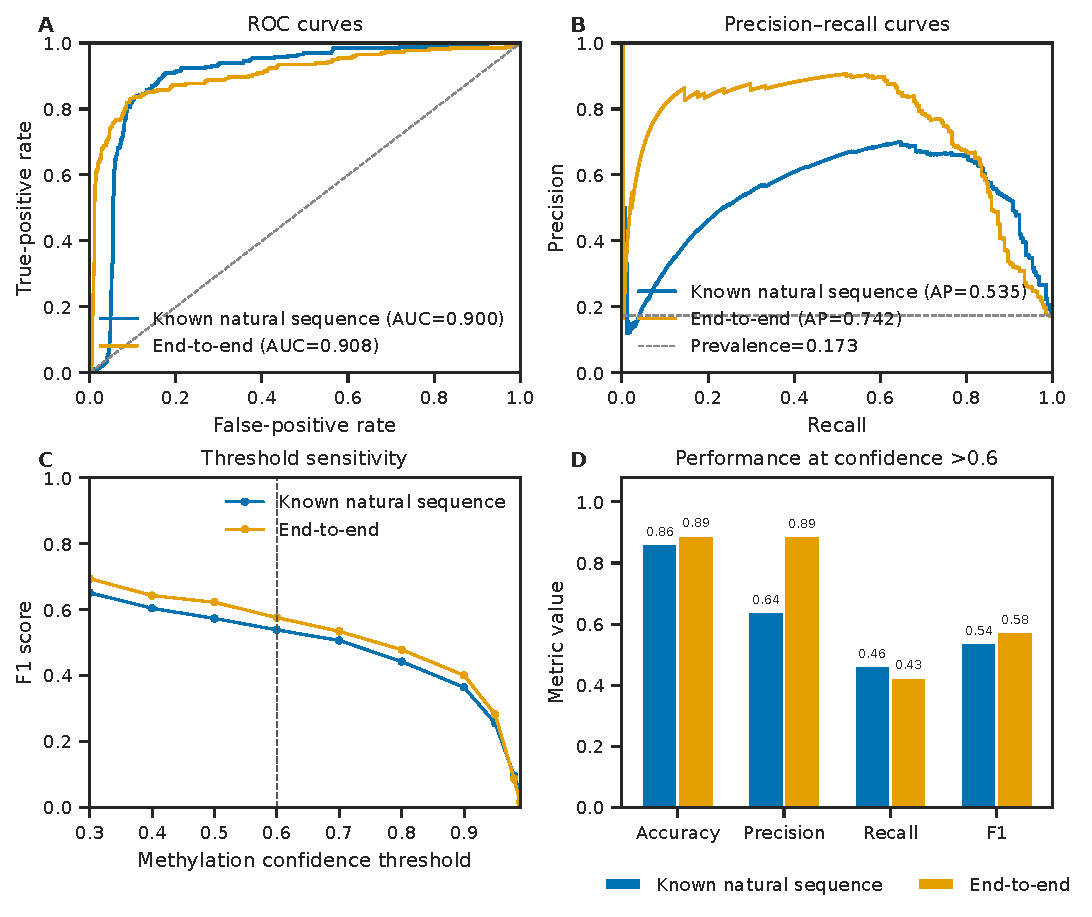
\includegraphics[width=0.98\textwidth]{figures/Fig4_original_checkpoint_model_performance.pdf}
  \caption{原始检查点在 Ser 来源修正单体留出集上的甲基化预测表现。A，ROC 曲线；B，精确率--召回率曲线；C，不同置信度阈值下的 F1；D，严格 $p>0.6$ 时的 Accuracy、Precision、Recall 与 F1。蓝色表示已知天然序列任务，橙色表示端到端任务。所有曲线和计数均来自1505个真实残基位点，不含 padding。}
  \label{fig:monomer-model-performance}
\end{figure}

\subsection{阈值结果的解释边界}

修正标签后，已知天然序列任务在阈值0.3处的 F1 高于阈值0.6，但0.3并非本文预设的部署阈值，而且该最大值是在同一留出集上观察得到。为避免用测试集反向挑选阈值，正文只报告预先冻结的严格 $p>0.6$ 结果，完整阈值敏感性由\cref{fig:monomer-model-performance}展示。若 RMC 表示端到端甲基阳性的二分类恢复，它等于 Recall，即 $111/261=42.53\%$；若要求真实甲基残基的天然氨基酸身份也正确，则为 $20/261=7.66\%$；若以全部位点为分母计算完整扩展 token 恢复，则为 $224/1505=14.88\%$。三者回答不同问题，本文不把它们混称为一个 RMC。

甲基二分类 Accuracy 较高也不等于完整序列设计准确。修正集阴性位点占82.66\%，而端到端 RAA 仅为16.08\%；只有联合 token 恢复率同时反映基础类别和甲基状态。正文因此并列报告 RAA、甲基分类指标和联合 token 恢复率，而不使用旧终端输出中的“Total End-to-End Acc”替代其中任何一项。

\subsection{原始 V28 没有可报告的单体结构结果}

单体 JSONL 中的坐标是 Rosetta 理论输入骨架，不是端到端设计序列的预测结构。现有 runbook 曾规划 explicit-methyl 与 naturalized 的 HighFold 结构任务，另有使用旧阈值0.30的参考/设计清单；但与本文阈值0.60相符的预测结构、成对结果表、PyRosetta 能量和通透性原始文件均不在可核验资产中。因此，原始 V28 的单体 CA/backbone/all-atom RMSD、甲基化位点 RMSD、pLDDT/pTM/PAE、能量、结构多样性和通透性均没有论文级数值。ipTM、界面 pLDDT、BSR 与受体框架姿态 RMSD对单链单体本身也不适用。上述项目明确记为“未计算/不适用”，而不是0；best85 或历史 V12 结果不得移植到 V28 单体队列。

\section{六个非3AV复合物：温度0.5的预设主分析}
\label{sec:results-six-complexes}

本节只报告原始 \path{frankenstein_v28.pt} 在六个非3AV复合物
（1SFI、3P8F、3WNE、3ZGC、4K1E和4KEL）上的结果。分析温度固定为
$T=0.5$；甲基化判定沿用生成文件中保存的严格规则 $p>0.6$，而不是
$p\geq 0.6$。所有比例均保留分子与分母，以区分两个回答不同问题的估计量：
保留后条件成功率以476条含至少一个甲基化标记的设计为分母，端到端产率则以
544条原始生成为分母。

\subsection{从原始生成到可评价队列}

在排除缓存目录中的重复文件后，六个靶点共得到544条原始序列；其中476条至少
含一个由严格阈值产生并保存为小写字母的甲基化标记，总体保留率为
$476/544=87.50\%$。保留率存在明显的靶点差异：1SFI、3P8F、4K1E和4KEL
均为$100/100$，3WNE仅为$27/84$，3ZGC为$49/60$（表~\ref{tab:six-raw-yield}）。
因此，单看保留后RMSD成功率会掩盖不同靶点生成有效甲基化序列的概率差异。

RMSD文件与生成记录采用“靶点名+区分大小写的设计序列”进行精确连接，476条
保留记录全部一一匹配（$476/476$），没有因模糊匹配、序列自然化或缺失RMSD
而删除样本。图~\ref{fig:task1-six-fig1}汇总了上述队列漏斗以及两种分母下的
通过情况。

\begin{table}[H]
  \centering
  \caption{六个非3AV复合物的序列漏斗与端到端联合RMSD产率}
  \label{tab:six-raw-yield}
  \small
  \begin{adjustbox}{max width=\textwidth}
  \begin{tabular}{lrrrrr}
    \toprule
    靶点 & 原始生成 & 保留 & 保留率 &
    \makecell{联合$<3\,\angstrom$\\（分子/原始生成）} &
    \makecell{联合$<5\,\angstrom$\\（分子/原始生成）} \\
    \midrule
    1SFI & 100 & 100 & 100.00\% & 1/100（1.00\%） & 19/100（19.00\%） \\
    3P8F & 100 & 100 & 100.00\% & 2/100（2.00\%） & 20/100（20.00\%） \\
    3WNE & 84  & 27  & 32.14\%  & 3/84（3.57\%）  & 5/84（5.95\%） \\
    3ZGC & 60  & 49  & 81.67\%  & 2/60（3.33\%）  & 23/60（38.33\%） \\
    4K1E & 100 & 100 & 100.00\% & 6/100（6.00\%） & 24/100（24.00\%） \\
    4KEL & 100 & 100 & 100.00\% & 2/100（2.00\%） & 10/100（10.00\%） \\
    \midrule
    \textbf{总体} & \textbf{544} & \textbf{476} & \textbf{87.50\%} &
    \textbf{16/544（2.94\%）} & \textbf{101/544（18.57\%）} \\
    \bottomrule
  \end{tabular}
  \end{adjustbox}
  \par\vspace{2pt}
  \footnotesize 注：端到端产率将未通过甲基化保留门槛的原始生成也计入分母；
  因而它同时反映“生成有效甲基化序列”和“结构通过联合阈值”两个步骤。
\end{table}

\begin{figure}[p]
  \centering
  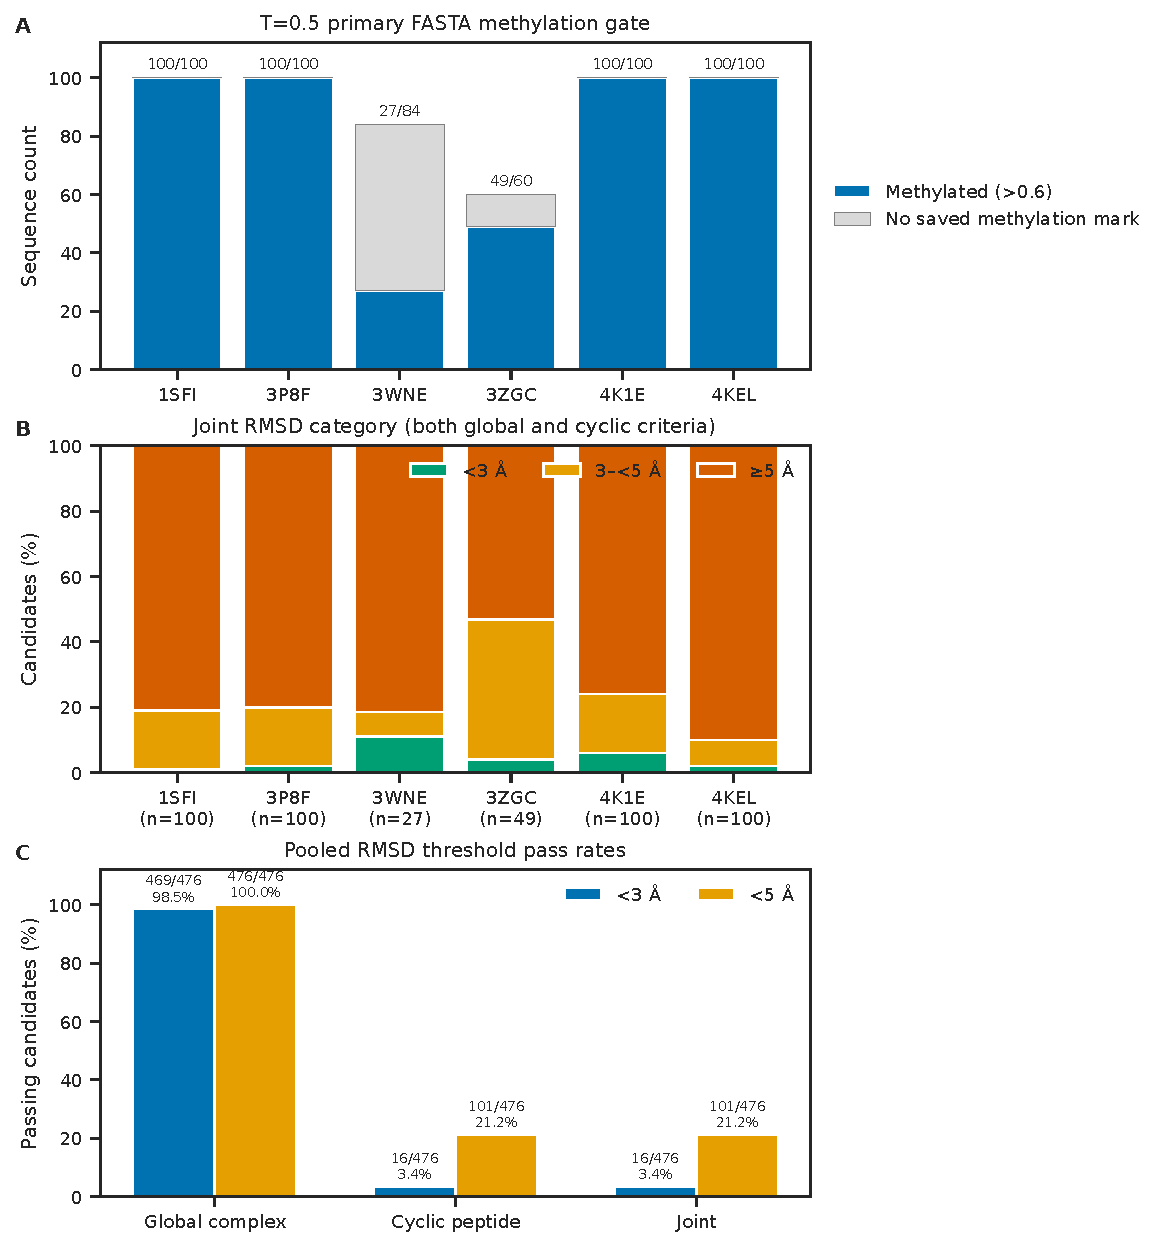
\includegraphics[width=0.98\textwidth]{figures/Fig1_cohort_and_rmsd_pass_rates.pdf}
  \caption{六个非3AV复合物的队列漏斗与RMSD通过率（Fig.~1）。
  （A）各靶点原始生成及严格$p>0.6$后保留数量；（B）各靶点联合RMSD类别；
  （C）总体全复合物、环肽以及二者联合的通过率。图中的结构通过率以476条
  保留设计为分母；从544条原始生成开始的端到端产率另见
  表~\ref{tab:six-raw-yield}。}
  \label{fig:task1-six-fig1}
\end{figure}

\subsection{RMSD分布与联合结构成功率}

按照预设口径，每个样本只进行一次全复合物CA叠合；随后在该坐标系内，对末链
环肽采用完整CA配对和最佳正向循环移位，不允许反向遍历，也不进行第二次肽链
单独拟合。联合通过要求同一条设计的全复合物CA RMSD与最佳正向循环肽CA RMSD
同时严格小于相应阈值。

在476条保留设计中，全复合物CA RMSD的总体中位数为
$1.022\,[0.692,1.534]~\angstrom$，最佳正向循环肽CA RMSD的总体中位数为
$6.738\,[5.261,8.129]~\angstrom$（中括号内为四分位距，表~\ref{tab:six-rmsd}）。
全复合物部分有$469/476=98.53\%$低于$3~\angstrom$，且$476/476=100\%$
低于$5~\angstrom$；因此总体失败主要由环肽在已经对齐的复合物坐标系中的
位置或构象偏差驱动，而不是受体整体叠合失败。

联合$<3~\angstrom$共有16条，保留后条件成功率为
$16/476=3.36\%$，95\% Wilson置信区间为$2.08\%$--$5.39\%$；联合
$<5~\angstrom$共有101条，条件成功率为$101/476=21.22\%$，95\% Wilson
置信区间为$17.78\%$--$25.11\%$。换用544条原始生成作分母时，对应端到端
产率分别为$2.94\%$（95\% Wilson置信区间$1.82\%$--$4.72\%$）和
$18.57\%$（$15.52\%$--$22.05\%$）。这两组数字不可互换：前者评价已生成
有效甲基化标记后的结构质量，后者回答一次原始生成最终得到合格设计的概率。

\begin{table}[H]
  \centering
  \caption{保留设计的RMSD分布与联合通过率}
  \label{tab:six-rmsd}
  \small
  \begin{adjustbox}{max width=\textwidth}
  \begin{tabular}{lrrrrr}
    \toprule
    靶点 & 保留数 &
    \makecell{全复合物CA RMSD\\中位数 [IQR]（\AA）} &
    \makecell{循环肽CA RMSD\\中位数 [IQR]（\AA）} &
    \makecell{联合$<3\,\angstrom$\\分子/保留数（\%）} &
    \makecell{联合$<5\,\angstrom$\\分子/保留数（\%）} \\
    \midrule
    1SFI & 100 & 0.884 [0.581, 1.457] & 6.289 [5.239, 7.814] & 1/100（1.00） & 19/100（19.00） \\
    3P8F & 100 & 0.981 [0.445, 1.364] & 6.375 [5.301, 7.282] & 2/100（2.00） & 20/100（20.00） \\
    3WNE & 27  & 0.904 [0.893, 0.927] & 29.002 [22.337, 39.916] & 3/27（11.11） & 5/27（18.52） \\
    3ZGC & 49  & 2.337 [1.662, 2.742] & 5.219 [4.367, 6.377] & 2/49（4.08） & 23/49（46.94） \\
    4K1E & 100 & 1.041 [0.691, 1.517] & 6.803 [5.071, 7.809] & 6/100（6.00） & 24/100（24.00） \\
    4KEL & 100 & 1.133 [0.701, 1.491] & 7.791 [6.361, 10.364] & 2/100（2.00） & 10/100（10.00） \\
    \midrule
    \textbf{总体} & \textbf{476} & \textbf{1.022 [0.692, 1.534]} &
    \textbf{6.738 [5.261, 8.129]} & \textbf{16/476（3.36）} &
    \textbf{101/476（21.22）} \\
    \bottomrule
  \end{tabular}
  \end{adjustbox}
  \par\vspace{2pt}
  \footnotesize 注：IQR为第25至第75百分位。表内百分比均以本靶点“保留数”为
  分母；总体$<3~\angstrom$与$<5~\angstrom$比例的95\% Wilson置信区间
  分别为$2.08\%$--$5.39\%$和$17.78\%$--$25.11\%$。
\end{table}

靶点层面的结果进一步说明为什么必须同时报告分子与分母。3WNE的环肽RMSD
中位数最高（$29.002~\angstrom$），但仍有$3/27$条低于$3~\angstrom$；由于其
仅保留27条，换成原始生成分母后为$3/84=3.57\%$。3ZGC的条件联合
$<5~\angstrom$比例最高（$23/49=46.94\%$），其端到端产率则为
$23/60=38.33\%$。这些描述性差异不应被解释为经多重比较校正后的靶点排名。
完整分布及两个RMSD之间的关系见图~\ref{fig:task1-six-fig2}。

\begin{figure}[p]
  \centering
  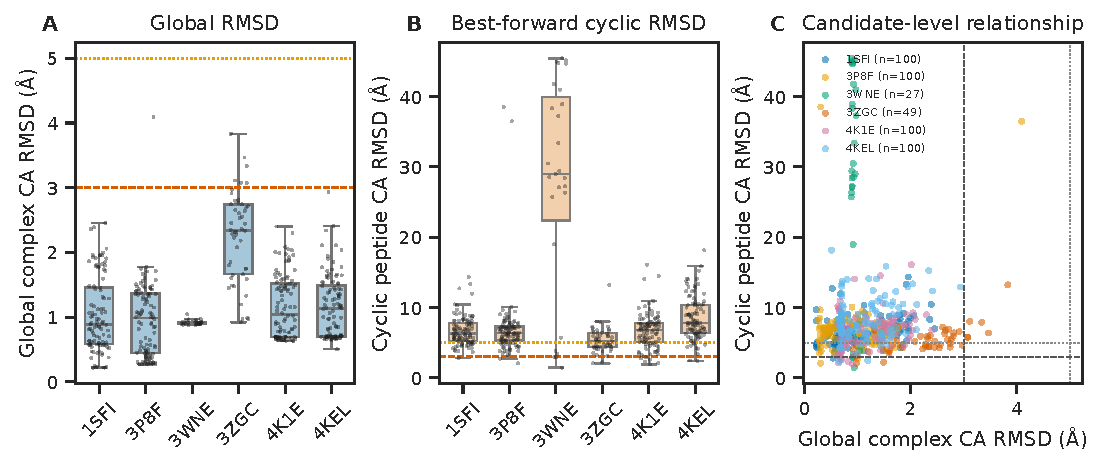
\includegraphics[width=0.98\textwidth]{figures/Fig2_rmsd_distributions.pdf}
  \caption{六个非3AV复合物的RMSD分布与关系（Fig.~2）。全复合物CA RMSD
  来自唯一一次全复合物叠合；循环肽CA RMSD在同一坐标系内采用最佳正向循环
  移位计算。虚线标示$3~\angstrom$与$5~\angstrom$阈值。}
  \label{fig:task1-six-fig2}
\end{figure}

作为表示方式敏感性分析，如果不允许循环移位而强制使用固定残基顺序，联合
$<3~\angstrom$和$<5~\angstrom$分别仅为$2/476=0.42\%$和
$33/476=6.93\%$；采用最佳正向循环移位后分别为$16/476=3.36\%$和
$101/476=21.22\%$。这一变化反映环状序列起点的表示等价性，并非重新生成或
重新拟合后的模型性能提升；主结果始终使用预先规定的最佳正向循环移位口径。

\subsection{甲基化输出的组成}

图~\ref{fig:task1-six-fig3}给出476条保留设计中甲基化位点和每条序列甲基化
数量的分布。这里的小写字母只是原始生成器在严格$p>0.6$规则下保存的预测
甲基化标记；它们不是实验测得的修饰状态，也不能据此推断真实酶学位点偏好。
该图的作用是描述进入RMSD分析的设计队列，而不是重新评价甲基化分类器的
独立准确率。

\begin{figure}[p]
  \centering
  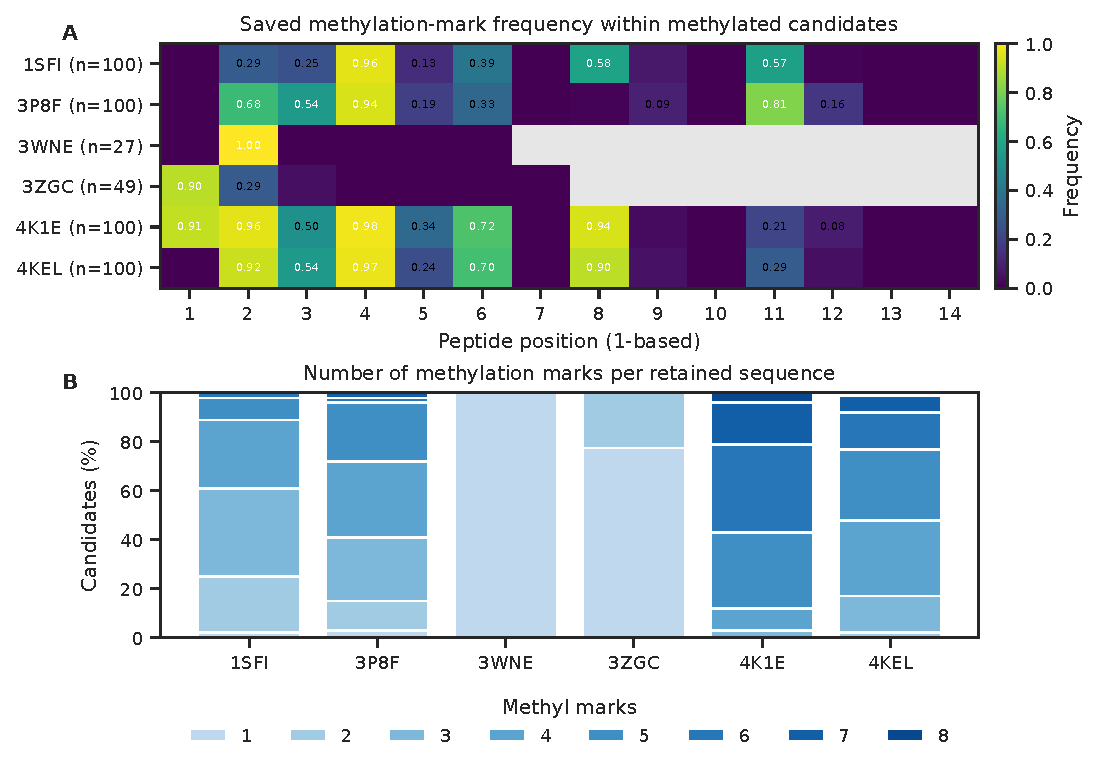
\includegraphics[width=0.98\textwidth]{figures/Fig3_methylation_positions_and_counts.pdf}
  \caption{保留设计的预测甲基化位置与数量（Fig.~3）。序列中的小写残基表示
  原始生成文件按严格$p>0.6$保存的甲基化预测；位点编号为设计肽链的1基坐标。}
  \label{fig:task1-six-fig3}
\end{figure}

\subsection{每靶点oracle代表与选择条件化的下游读数}

为便于逐个靶点查看具体序列，从每个靶点的保留设计中选取最佳正向循环肽CA
RMSD最小的一条，得到六条oracle代表（表~\ref{tab:six-oracle}）。六条代表的
循环肽RMSD均低于$3~\angstrom$，但这一事实是选择规则的直接结果，不能代替
随机或预先固定候选上的成功率估计。图~\ref{fig:task1-six-fig5}汇总这些代表的
RMSD、预测通透性、固定构象PyRosetta界面能以及结构文件CA B-factor均值代理量。

\begin{table}[H]
  \centering
  \caption{六个靶点按最小循环肽RMSD选择的oracle代表}
  \label{tab:six-oracle}
  \scriptsize
  \begin{adjustbox}{max width=\textwidth}
  \begin{tabular}{llrrrrrr}
    \toprule
    靶点 & 设计序列 & 甲基化位点 &
    \makecell{全复合物\\RMSD（\AA）} &
    \makecell{循环肽\\RMSD（\AA）} &
    \makecell{预测通透性\\（模型单位）} &
    \makecell{固定构象\\界面能（REU）} &
    \makecell{CA B-factor\\均值代理量} \\
    \midrule
    1SFI & \seq{RCCrGNCGQCQFGG} & 4 & 0.536 & 2.818 & $0.454$ & 31.77 & 93.49 \\
    3P8F & \seq{CrrrGrQGKGrRGC} & 2,3,4,6,11 & 0.300 & 2.075 & $7.57\times10^{-35}$ & $-25.73$ & 91.57 \\
    3WNE & \seq{GrKWNC} & 2 & 0.933 & 1.459 & $0.0864$ & 0.73 & 90.03 \\
    3ZGC & \seq{rEGGQNR} & 1 & 0.973 & 2.076 & $1.04\times10^{-7}$ & 15.95 & 89.91 \\
    4K1E & \seq{rcrrrQCrQGNCDR} & 1,2,3,4,5,8 & 0.900 & 1.916 & $6.14\times10^{-32}$ & 434.24 & 89.04 \\
    4KEL & \seq{RcrrGNCrQGFCDR} & 2,3,4,8 & 0.655 & 2.379 & $0.00214$ & 416.77 & 91.49 \\
    \bottomrule
  \end{tabular}
  \end{adjustbox}
  \par\vspace{2pt}
  \footnotesize 注：每行均在观察该靶点全部候选的循环肽RMSD后再选择，故所有
  后续读数均为选择条件化描述。CA B-factor均值只是相应结构文件字段的代理量，
  不应与来自另一流程、另一标定方式的pLDDT直接等同。通透性列没有实验标签，
  也没有校准到物理单位。
\end{table}

\begin{tcolorbox}[colback=SoftAmber,colframe=Amber,title={oracle选择警告}]
表~\ref{tab:six-oracle}中的序列并非预先指定，也不是从476条设计中随机抽取；
它们是在观察目标结局——循环肽RMSD——之后逐靶点取最小值。因此，代表序列
及图~\ref{fig:task1-six-fig5}中的下游指标只能用于候选展示和后续验证优先级，
不能用于估计模型的总体成功概率，也不能把六条代表的均值当作未选择队列的
无偏性能。通透性预测同样是在该选择之后报告，应视为探索性结果。固定构象
PyRosetta界面能未经过统一松弛或重打包，而结构文件中的
\path{highfold_ca_bfactor_mean}仅作置信度代理；二者均不构成实验结合或稳定性
证据。无选择偏倚的成功率应以表~\ref{tab:six-raw-yield}和
表~\ref{tab:six-rmsd}中的全部544条或476条记录为准。
\end{tcolorbox}

\begin{figure}[p]
  \centering
  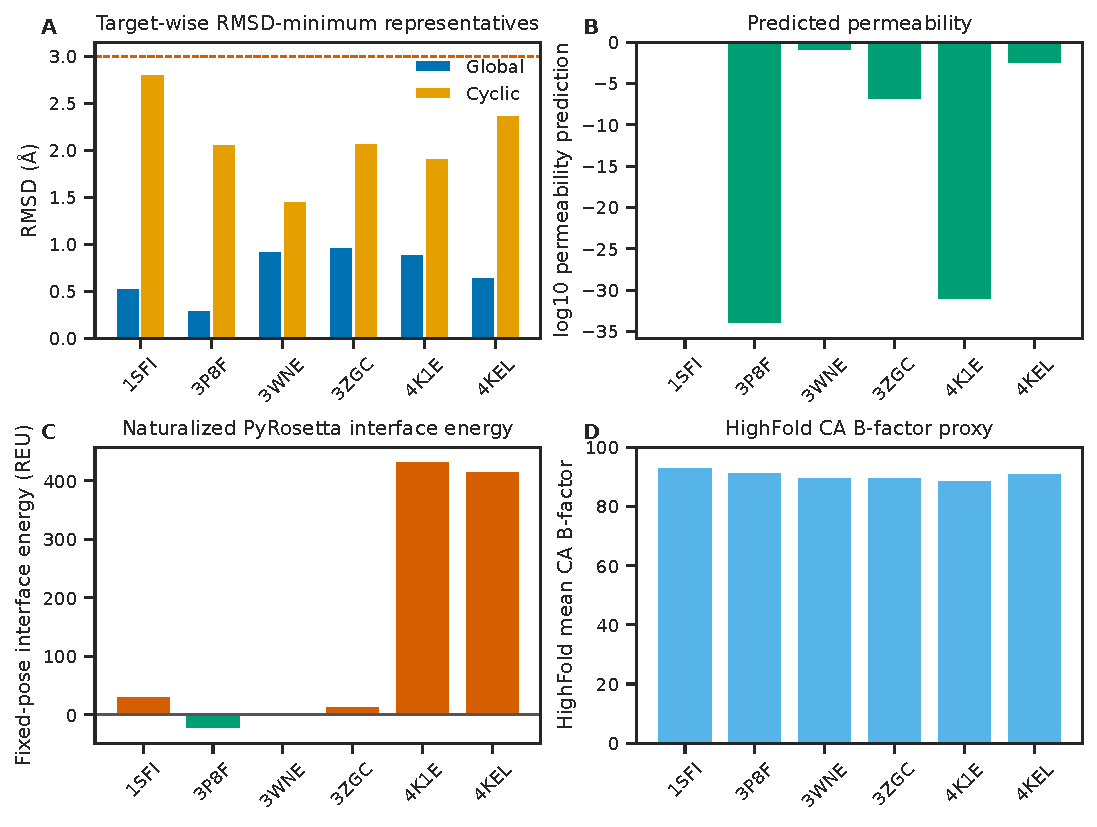
\includegraphics[width=0.98\textwidth]{figures/Fig5_selection_conditioned_downstream_metrics.pdf}
  \caption{六条oracle代表的选择条件化下游指标（Fig.~5）。（A）全复合物与
  循环肽RMSD；（B）预测通透性（log10尺度）；（C）固定构象PyRosetta界面能；（D）结构
  文件CA B-factor均值代理量。所有面板均须结合正文的oracle选择警告解释。}
  \label{fig:task1-six-fig5}
\end{figure}

\section{17 靶点的探索性支持结果}

\subsection{天然复合物集合不能评价甲基阳性召回}

17 个天然复合物共包含251个选中短肽位点；天然结构的序列评价保留预先选定的全部短肽链，部分靶点因此贡献多条等价肽链，而生成结构评价只使用单条预测末链。天然化基础序列恢复为 53/251（21.12\%）。这251个真值位点全部是未甲基化阴性，因此 ROC-AUC、Precision、Recall 和 F1 都没有阳性类别可供计算；若给出这些数字，数学上没有意义。阈值严格 $p>0.6$ 时，已知天然序列条件产生 19 个假阳性（19/251，7.57\%），端到端条件产生 9 个预测甲基位点（9/251，3.59\%）。后一个比例同时受基础氨基酸预测错误影响，不能解释为甲基化头单独的假阳性率。

\begin{table}[H]
\centering
\caption{17 个天然复合物上的可报告序列指标。所有甲基化真值均为阴性。}
\label{tab:native17}
\begin{tabular}{L{47mm}C{29mm}C{29mm}L{44mm}}
\toprule
指标 & 计数 & 比例 & 解释 \\
\midrule
天然化 RAA & 53/251 & 21.12\% & 基础氨基酸恢复 \\
已知序列甲基假阳性 & 19/251 & 7.57\% & 真阴性集合上的 FPR \\
端到端预测甲基位点 & 9/251 & 3.59\% & 含基础类别级联误差 \\
AUC/Precision/Recall/F1 & \NA & 不可定义 & 没有甲基阳性真值 \\
\bottomrule
\end{tabular}
\end{table}

\subsection{五个温度的生成覆盖与重复率}

原始全温度文件共有 4015 条记录；分别在每个温度内去重后合计 3443 条。比较两个端点，温度内唯一率在 $T=0.01$ 与0.5时分别为78.05\%和94.88\%，平均天然序列恢复分别为1.49\%和4.42\%，平均甲基标记率分别为27.69\%和9.67\%（\cref{tab:alltemp}）。其中唯一率在 $T=0.1$ 降至74.37\%，所以这些变化并非全程单调。它们是生成池的描述统计，不是独立同分布实验重复，也不能把不同温度的样本量差异解释为温度效应的因果证据。

\begin{table}[H]
\centering
\caption{17 靶点原始生成池的温度分层统计。唯一数是在各温度内去重；甲基标记率为序列内小写甲基 token 比例的均值。}
\label{tab:alltemp}
\begin{tabular}{C{15mm}rrrrrr}
\toprule
$T$ & 原始数 & 唯一数 & 重复数 & 唯一率 & 平均 RAA & 平均甲基率 \\
\midrule
0.01 & 82   & 64   & 18  & 78.05\% & 1.49\% & 27.69\% \\
0.10 & 394  & 293  & 101 & 74.37\% & 2.46\% & 23.24\% \\
0.20 & 776  & 597  & 179 & 76.93\% & 3.52\% & 19.87\% \\
0.30 & 1181 & 988  & 193 & 83.66\% & 3.90\% & 15.54\% \\
0.50 & 1582 & 1501 & 81 & 94.88\% & 4.42\% & 9.67\% \\
\midrule
合计 & 4015 & 3443 & 572 & 85.75\% & \NA & \NA \\
\bottomrule
\end{tabular}
\end{table}

\subsection{best85：肽内部形状尚可，但结合姿态普遍偏离}

旧 best85 队列覆盖 $17\times5=85$ 个靶点--温度组合，结构文件和链映射均为 85/85。由于每个组合的代表是按真实天然序列恢复率从多个候选中选出，这一队列是选择条件化的 oracle 集合；它回答“知道天然答案后所挑代表的表现”，不回答一次盲生成的期望表现。

在受体框架对齐后，肽 CA RMSD 的均值/中位数为 29.93/40.06~\AA，肽 backbone RMSD 为 29.83/39.96~\AA；CA RMSD $<2$~\AA 为 0/85，$<5$~\AA 为 3/85（3.53\%）。相反，单独对肽自身拟合后，CA 与 backbone RMSD 的均值/中位数分别为 2.65/2.53~\AA 和 2.34/2.11~\AA（\cref{tab:best85-rmsd}）。这组巨大差异说明，部分序列可形成与天然肽相似的内部形状，但没有位于正确的受体结合位置；因此不能用肽自对齐 RMSD 宣称设计成功。

\begin{table}[H]
\centering
\caption{best85 的旧结构评价。受体框架对齐反映结合姿态；肽自对齐仅反映内部形状。}
\label{tab:best85-rmsd}
\begin{tabular}{L{58mm}C{20mm}C{23mm}C{29mm}}
\toprule
指标 & $n$ & 均值（\AA） & 中位数（\AA） \\
\midrule
受体拟合后肽 CA RMSD & 85 & 29.930 & 40.064 \\
受体拟合后肽 backbone RMSD & 85 & 29.835 & 39.960 \\
肽自拟合 CA RMSD & 85 & 2.647 & 2.530 \\
肽自拟合 backbone RMSD & 85 & 2.342 & 2.105 \\
\bottomrule
\end{tabular}
\end{table}

best85 共含 159 个模型标记的甲基位点和 626 个非甲基位点。按两组坐标平方和合并后开方得到的 pooled CA RMSD，在受体拟合后分别为20.43与34.18~\AA，在肽自拟合后分别为3.28与2.93~\AA；这些数值不是逐设计或逐位点 RMSD 的算术均值。由于位点是否甲基化本身由模型选择，并同时关联残基类别、靶点、温度和结构可解析性，这只是选择后的描述，不能推出“甲基化导致更好结合姿态”或其他因果关系。

\subsection{多样性、置信度、通透性和 fixed-pose 分数}

同一靶点的五个温度代表进行两两比较，共得到170对。对称 TM-score 的均值与中位数分别为0.340和0.309；对应多样性 $1-\mathrm{TM}$ 分别为0.660和0.691，提示代表结构之间存在较大内部形状差异。但它既受温度影响，也受 oracle 挑选影响，不等价于完整生成分布的多样性。

结构 PDB 的 CA B-factor 代理在 85/85 条中可用，均值为 87.55。HighFold COMMENT 的 global pLDDT、肽链 pLDDT、pTM 和受体--肽 ipTM/PAE 字段仅在 37/85 条中存在；在这些可用条目中，global pLDDT、肽链 pLDDT、pTM 与受体--肽 ipTM 的均值分别为 71.07、46.53、0.146 和 0.461，肽链内 PAE、链间 PAE 与界面 PAE 的均值分别为 3.64、18.05 和 12.14。缺失的 48 条不能填零，PDB B-factor 代理也不能替代 COMMENT 字段。

预测通透性在85/85条中有数值：82条由靶点、序列和温度严格匹配，3条（3WNE 的 $T=0.01/0.1$ 与3ZGC的 $T=0.1$）因同一序列跨温度重复而回填，故温度分层图包含这项来源限制。总体中位数为 $1.84\times10^{-8}$（模型单位）；两个端点 $T=0.01$ 与0.5的中位数分别为 $3.17\times10^{-9}$ 与 $5.16\times10^{-6}$，但 $T=0.1$ 为 $2.43\times10^{-9}$，并非全程单调。由于没有实验通透性标签，这只能视为模型预测分布，不能报告准确率或外部验证结论。

自然化 fixed-pose PyRosetta 评分覆盖 85/85 条。复合物每残基分数的中位数为 1.799~REU，cross-interface 分数的均值/中位数为 259.97/110.07~REU，只有 6/85 为负。该流程没有在同一参数化、同一优化协议下计算天然参考，也没有显式 N-甲基残基参数；因此无法计算“低于天然能量”的 success 或 stability，更不能把这些数值称为结合自由能。

\begin{figure}[H]
  \centering
  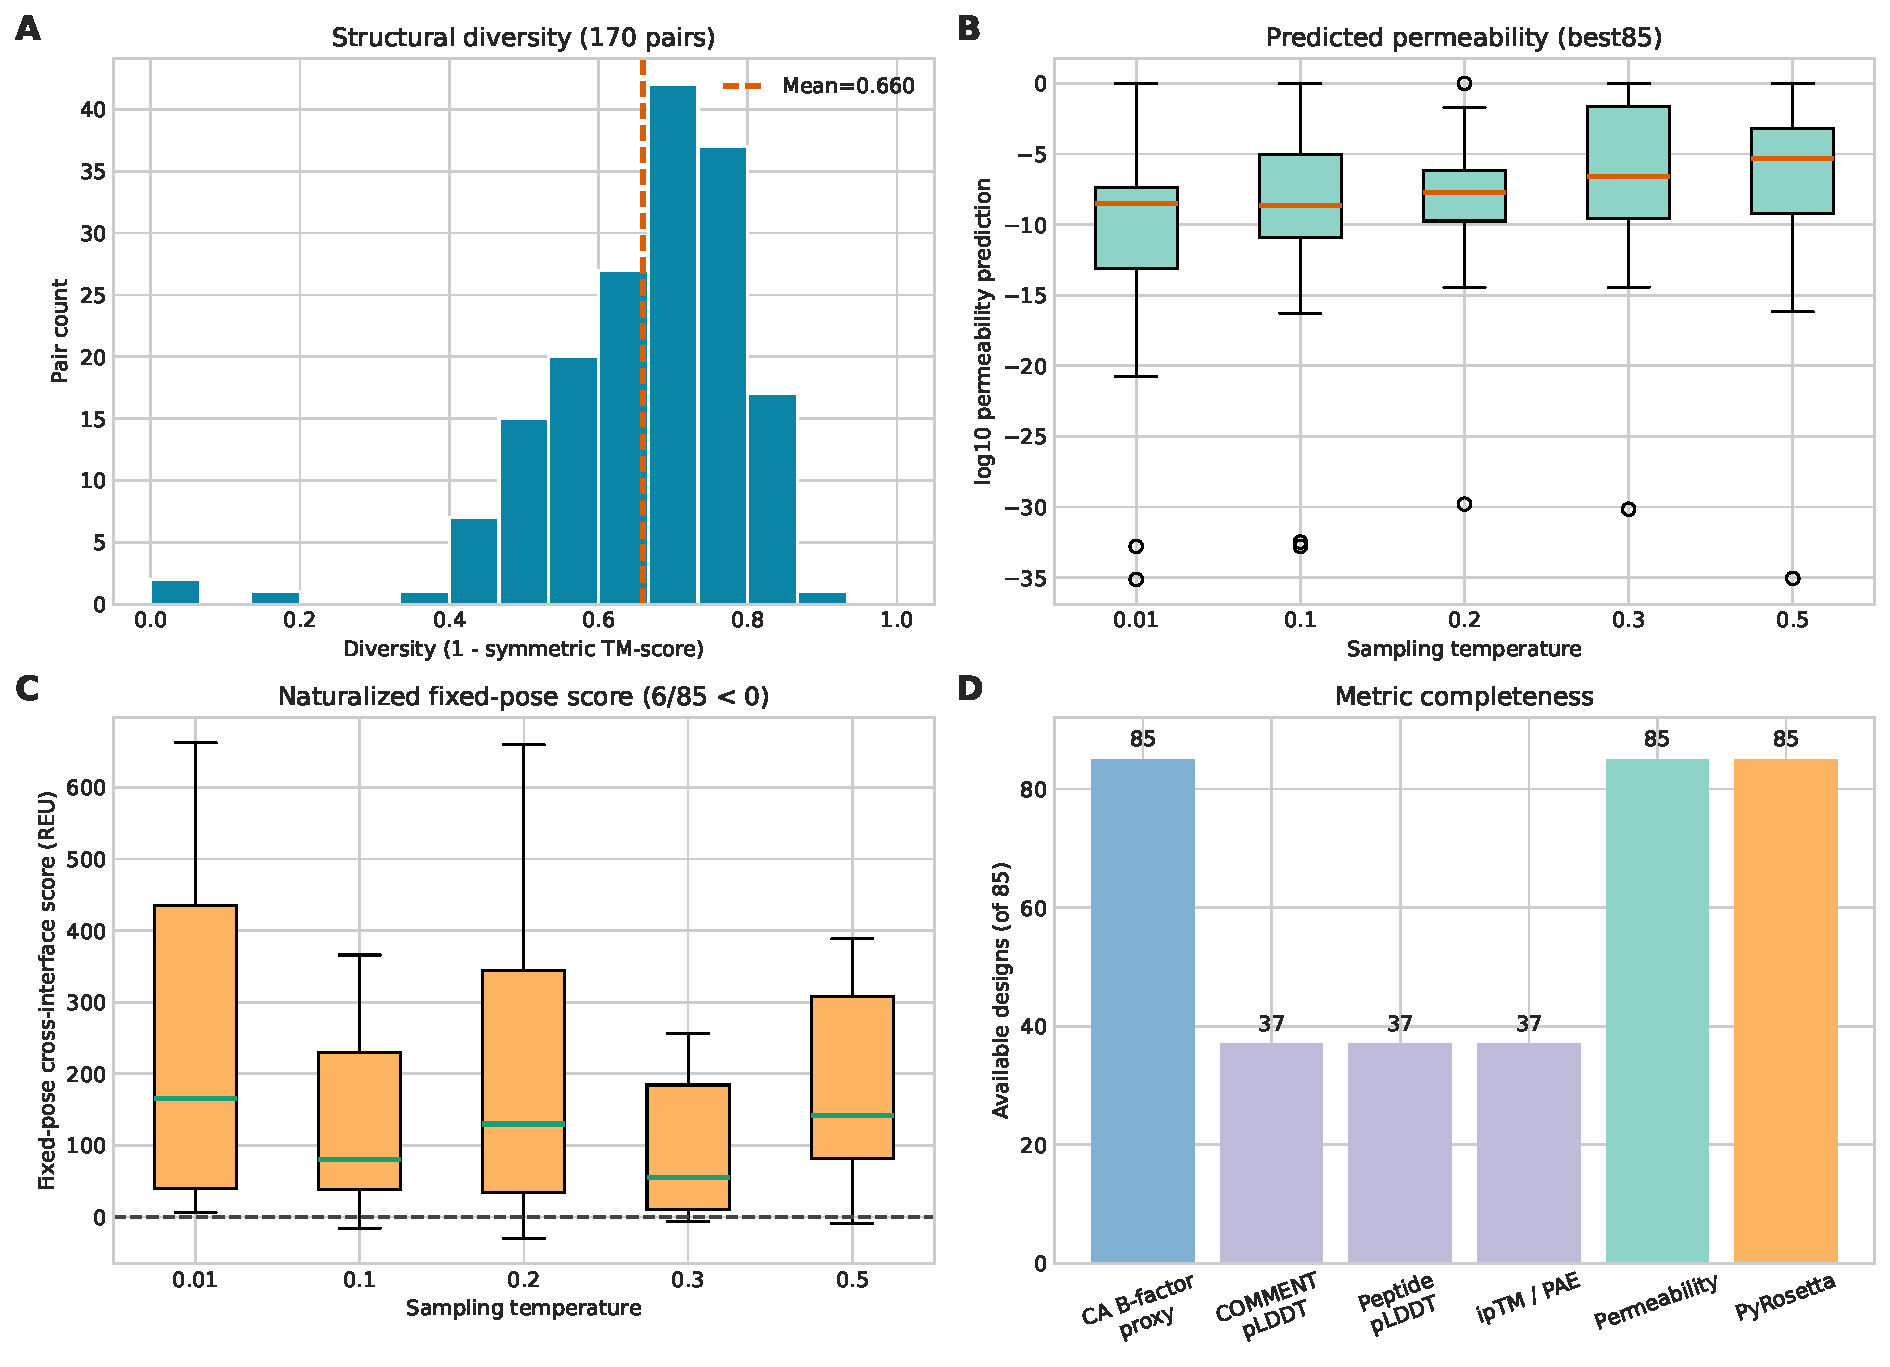
\includegraphics[width=0.98\textwidth]{figures/Fig6_best85_exploratory_support.pdf}
  \caption{17 靶点 best85 的探索性支持结果。A，靶点内五温度代表的 $1-\mathrm{TM}$ 分布；B，按温度分层的通透性预测，其中3条为相同序列的跨温度回填；C，自然化 fixed-pose cross-interface Rosetta 分数；D，各指标的文件可用数。所有面板均受 oracle 选择影响，不能替代六复合物的预设主分析。}
  \label{fig:best85}
\end{figure}

\section{讨论}

\subsection{原始模型的能力边界}

本次统一审计显示，原始 Frankenstein-v28 的甲基化头并非完全失效：修正真值后，已知序列与端到端 AUC 仍分别达到 0.900 和 0.908，说明预测分数对阳性、阴性位点具有排序信息。然而，固定在项目预设阈值 $>0.6$ 时，Recall 只有 46.36\% 和 42.53\%，意味着超过一半真实甲基位点没有被保留。与此同时，天然化 RAA 只有 16.08\%，所以“甲基分类不错”和“完整扩展氨基酸序列恢复好”不能互相替代。

六个非 3AV 复合物给出了更接近实际筛选流程的答案。544 条温度 0.5 原始序列中，476 条通过甲基保留门；联合 RMSD $<5$~\AA 的最终端到端产率为 18.57\%，$<3$~\AA 为 2.94\%。如果只对 476 条保留样本报告 21.22\% 和 3.36\%，会忽略甲基门带来的损失，因此本文同时固定两个分母。

结构误差的主要来源也很清楚：476 条中 469 条全局复合物 CA RMSD $<3$~\AA、全部 476 条 $<5$~\AA，但联合通过数只有 16 和 101。换言之，瓶颈不是整体受体框架，而是同一全局坐标系内的环肽结合姿态。best85 中“肽自拟合约 2.65~\AA、受体框架拟合后约 29.93~\AA”的差距从另一队列支持了同一解释，但因选择方式和 RMSD 定义不同，不能把两个队列合并计算。

\subsection{不同靶点需要不同诊断}

六个靶点没有表现出统一失败模式。3WNE 的甲基保留率只有 27/84（32.14\%），且保留后环肽 RMSD 中位数达到 29.00~\AA，甲基门和结合姿态都是瓶颈。3ZGC 的保留率为 49/60（81.67\%），联合 $<5$~\AA 的原始产率达到 38.33\%，但其全局 RMSD 中位数 2.34~\AA 高于其他靶点，提示整体结构拟合仍需关注。1SFI、3P8F、4K1E 和 4KEL 全部通过甲基保留门，但联合 $<5$~\AA 的原始产率仍只有 10--24\%，说明仅提高甲基标记概率并不能解决姿态问题。

因此，后续模型改进不宜只优化一个总体 Accuracy。更合理的错误分解是：基础残基类别、甲基化判断、完整序列有效率、受体框架质量、环肽内部形状和环肽结合姿态分别追踪，并按靶点报告。只有这样才能判断修改真正修复了哪一步。

\subsection{数据审计为何改变结论}

旧单体标签把 62 个 Ser 错列为甲基阳性，旧评价脚本又把批次 padding 的零初始化位置当作真实阴性。前一个问题改变真值，后一个问题使结果依赖 batch size。两者都会产生表面上更好、却不可复现的 Accuracy 或 F1。本文没有改变检查点和位点预测概率，只修正评价标签并限制到 1505 个真实位点，因此主结果应视为对同一模型的更干净估计，而不是一次新的训练结果。

数据来源审计还改变了单体集合的性质判断。规划截图提出了 ``Baker 33'' 和 ``Rosetta 400+300''，但逐文件复核显示 751/751 个原始 PDB 均声明为 Rosetta 理论模型，其中406个来自 Rosetta-2023、345个来自 Rosetta-2025；没有找到可核验的 Baker 33 实验结构子集。因此，截图应被视为早期规划，而不能覆盖冻结数据本身。当前仍缺少的是 checkpoint 的完整训练 manifest 与同源聚类级泄漏审计，而不是这些 PDB 的 Rosetta 理论来源。

\subsection{限制与尚未完成的论文指标}

本稿的主要限制如下：

\begin{enumerate}
  \item 151 个单体没有与原始 V28 一一对应的预测结构结果，因此不能报告单体 CA/backbone/all-atom RMSD、pLDDT、能量或通透性。历史 164 条结构表属于 V12 工作流，不能移植到 V28。
  \item 六复合物主分析有 CA 层面的全局与环肽 RMSD，但没有统一可用的 backbone/all-atom 甲基化 RMSD、结合位点恢复、同靶点完整多样性或原生对照能量。
  \item best85 使用真实天然序列恢复率挑选，存在 oracle 选择偏倚；其结果不能代表盲生成或 100 条/靶点的未来批次。
  \item 置信度、通透性与 Rosetta 分数均为计算量，尚无实验结构、实验通透性、亲和力或稳定性验证。
  \item 主要比例来自 6 个靶点，靶点间异质性明显；逐序列 Wilson 区间不包含靶点抽样不确定性。
  \item 本稿为既有文件的回顾性整合，没有重新运行上游模型；这保证了口径唯一，但无法补回从未生成的指标。
\end{enumerate}

\subsection{下一步最小充分验证}

对后续修复模型，建议保持本稿所有阈值和分母不变，先在 17 个复合物每靶点 100 条的盲生成集上冻结序列，再统一生成结构。预先登记的主要终点应是：原始生成分母上的含甲基有效率、全局对齐后环肽姿态 RMSD $<3$ 和 $<5$~\AA 比例；次要终点才是肽自拟合 RMSD、置信度、多样性、通透性预测和同协议天然对照能量。模型修复前后必须使用相同靶点、随机种子规划、结构生成器版本和 RMSD 脚本，且禁止用天然序列恢复率挑选代表。只有这一步通过，才适合扩大到每靶点 1000 条。

\section{结论}

本研究把原始 \path{frankenstein_v28.pt} 的单体和复合物证据首次统一到一个可追溯口径。Ser 来源修正后，模型的甲基化排序能力仍然存在，但固定阈值下召回有限，且基础序列恢复率较低。六个非 3AV 复合物在温度 0.5、严格甲基置信度 $>0.6$ 下，从 544 条原始生成出发，联合 RMSD $<3$ 和 $<5$~\AA 的端到端产率分别为 2.94\% 与 18.57\%；环肽结合姿态是主要结构瓶颈。

17 靶点 best85 的多样性、置信度、通透性和 fixed-pose 能量提供了探索性背景，但其 oracle 选择和指标缺失不允许把它解释为部署成功率。尚无原始 V28 单体结构结果，也尚无统一的全原子甲基 RMSD、BSR、相对天然能量 success/stability 或实验通透性。因而，本稿适合作为后续 V8 修复和 1700 条盲生成验证的冻结基线，而不是终点性能宣称。


\clearpage
\appendix
\section{尚哥指标清单的证据可用性矩阵}
\label{app:metric-matrix}

本附录逐项对应尚哥提供的模型、数据和指标提纲。全文涉及的五层分母严格分开：
\begin{enumerate}
  \item \textbf{单体：}Ser 来源修正留出集，151条、1505个真实位点，正文阈值严格 $p>0.6$；
  \item \textbf{六复合物主分析：}六个非 3AV 靶点、$T=0.5$、544条原始序列和476条甲基化保留候选；
  \item \textbf{天然17靶点：}预先选定的全部短肽链，共251个天然位点；
  \item \textbf{17靶点全温度生成池：}五个温度共4015条原始记录、3443条温度内唯一序列；
  \item \textbf{best85 探索集：}17个靶点、五个温度、按天然序列恢复率选择的85个 oracle 代表。
\end{enumerate}

状态含义如下：\textbf{可报告}表示定义、分母和来源均已冻结；\textbf{探索性}表示数值存在，但受 oracle 选择、预测模型或非实验代理限制；\textbf{不可定义}表示真值类别缺失，数学上不能计算；\textbf{未计算}表示没有合格的成对数据或冻结定义。任何“不可定义/未计算”均不等于数值0。

\subsection{模型、数据与序列指标}

\begin{landscape}
\begingroup
\small
\setlength{\tabcolsep}{3pt}
\renewcommand{\arraystretch}{1.22}
\begin{longtable}{L{27mm}L{46mm}L{50mm}L{48mm}L{43mm}}
\caption{模型、数据与序列指标的队列级可用性。}\label{tab:metric-matrix-sequence}\\
\toprule
清单项目 & 单体 & 六复合物主分析 & \makecell{17靶点探索\\（天然/生成/best85）} & 状态与原因 \\
\midrule
\endfirsthead
\multicolumn{5}{l}{\small\itshape 表\thetable（续）}\\
\toprule
清单项目 & 单体 & 六复合物主分析 & \makecell{17靶点探索\\（天然/生成/best85）} & 状态与原因 \\
\midrule
\endhead
\midrule
\multicolumn{5}{r}{\small 接下页}\\
\endfoot
\bottomrule
\endlastfoot

基于甲基化单体的微调
& 冻结检查点可评价；历史审计记录 train/test 为600/151，但无原始训练全过程日志、随机种子曲线和相对于初始化模型的配对增益
& 使用同一冻结检查点生成/评分，不构成新的训练证据
& 天然集、全温度池和 best85 均使用同一冻结检查点；oracle 选择不能反推微调增益
& \textbf{部分可报告}：可写模型和检查点，不可编造“微调提高了多少” \\

甲基化分类器
& known-sequence 与 end-to-end 均有261阳性/1244阴性真值
& 75个天然位点全为阴性；476条生成序列无实验甲基真值
& 天然251位点全为阴性；全温度池和85条代表只有模型小写标记，无实验甲基真值
& 单体\textbf{可报告}；复合物生成序列只能报告标记/保留率 \\

Baker 33 个真结构单体
& 未找到；751/751 个原始 PDB 均标记为 Rosetta 理论模型，没有可核验的 Baker 实验结构子集
& 不适用
& 不适用
& \textbf{与冻结数据不符}：不得把规划数字写成已完成数据 \\

Rosetta 400+300 个单体
& 实际为406个 Rosetta-2023 与345个 Rosetta-2025 理论模型，合计751；训练/测试为600/151
& 不适用
& 不适用
& \textbf{可报告实际构成}：规划的400+300数字不采用 \\

17 个真结构复合物
& 不适用
& 从17个靶点中预设选取六个非3AV靶点
& 天然17靶点用于序列评价；best85为85/85结构匹配
& \textbf{可报告}，但六靶点与 best85 的队列和 RMSD 定义不同 \\

RAA（天然化氨基酸恢复）
& $242/1505=16.08\%$
& 天然六复合物七条选定肽链为 $29/75=38.67\%$；不得与476条生成候选的回收字段混为同一测试
& 天然17靶点为$53/251=21.12\%$；全温度池按温度的平均RAA为1.49--4.42\%；best85的 recovery 是 oracle 选择标准
& 单体、天然六复合物和天然17靶点\textbf{可报告}；生成池为描述性，best85有\textbf{选择偏倚} \\

AUC
& known-sequence 0.9003；end-to-end 0.9082
& 天然75位点阳性数为0，AUC不可定义；生成476条无实验真值
& 天然251位点无阳性，AUC不可定义；生成池与best85无实验甲基真值
& 仅单体\textbf{可报告} \\

Accuracy（严格 $p>0.6$）
& known $1297/1505=86.18\%$；end-to-end $1341/1505=89.10\%$
& 天然阴性集 known $71/75=94.67\%$；end-to-end $73/75=97.33\%$，实质为 $1-\mathrm{FPR}$；生成476条不可计算
& 天然17靶点 known $232/251=92.43\%$、end-to-end $242/251=96.41\%$，实质为$1-\mathrm{FPR}$；生成池与best85不能计算
& 单体\textbf{可报告}；两个天然复合物阴性集仅作误报审计 \\

Precision / Recall / F1
& known 64.02\%/46.36\%/53.78\%；end-to-end 88.80\%/42.53\%/57.51\%
& 天然位点无阳性，三项不可定义；生成候选无真值
& 天然251位点无阳性，三项不可定义；生成池与best85无实验真值
& 仅单体\textbf{可报告} \\

RMC
& 二分类甲基召回 $111/261=42.53\%$；端到端真实甲基残基身份完全恢复 $20/261=7.66\%$；全部位点联合 token 恢复 $224/1505=14.88\%$
& 同理；因无阳性，不能把RMC写成0
& 天然251位点无阳性，不能把RMC写成0；生成池与best85无真值
& \textbf{术语歧义}：必须同时写明身份要求与分母 \\

FPR / 预测阳性率
& known FPR 5.47\%、预测阳性率12.56\%；end-to-end 1.13\%、8.31\%
& 天然阴性集 known $4/75=5.33\%$；end-to-end $2/75=2.67\%$
& 天然17靶点 known FPR $19/251=7.57\%$；end-to-end预测阳性率$9/251=3.59\%$；生成池可统计小写率但不能称FPR
& 单体及两个天然阴性集\textbf{可报告} \\

联合扩展 token 恢复
& 基础类别与甲基状态同时正确：$224/1505=14.88\%$
& 未形成可复核的75位点联合交叉表；生成候选无扩展 token 真值
& 天然17靶点未形成联合交叉表；生成池与best85无扩展 token 真值
& 仅单体\textbf{可报告}；不能用 RAA 与 Accuracy 相乘替代 \\

甲基化保留率/有效生成概率
& 不适用；这是生成队列指标
& $476/544=87.50\%$ 含至少一个严格 $p>0.6$ 的已保存小写标记；联合 $<3$/$<5$ 原始产率为 $16/544=2.94\%$、$101/544=18.57\%$
& 全温度池有4015条记录，但未定义与主队列相同的端到端结构成功门；best85固定为85个oracle代表
& 六复合物\textbf{主结果可报告} \\

旧标签/旧 padding 阈值截图
& 不进入正文；旧标签含62个Ser来源错误，旧截图分母随 batch size 改变
& 不适用
& 不适用
& \textbf{仅历史审计}：不可与本表正文指标并列 \\

\end{longtable}
\endgroup
\end{landscape}

\subsection{结构、能量、多样性与通透性指标}

\begin{landscape}
\begingroup
\footnotesize
\setlength{\tabcolsep}{3pt}
\renewcommand{\arraystretch}{1.20}
\begin{longtable}{L{29mm}L{43mm}L{51mm}L{52mm}L{40mm}}
\caption{结构与下游指标的队列级可用性。}\label{tab:metric-matrix-structure}\\
\toprule
清单项目 & 单体 & 六复合物主分析 & \makecell{17靶点探索\\（天然/生成/best85）} & 状态与原因 \\
\midrule
\endfirsthead
\multicolumn{5}{l}{\small\itshape 表\thetable（续）}\\
\toprule
清单项目 & 单体 & 六复合物主分析 & \makecell{17靶点探索\\（天然/生成/best85）} & 状态与原因 \\
\midrule
\endhead
\midrule
\multicolumn{5}{r}{\small 接下页}\\
\endfoot
\bottomrule
\endlastfoot

RMSD\_CA
& 无端到端单体设计结构--参考结构配对
& 476/476有一次全复合物对齐后的全局 CA 与末链 best-forward 环肽 CA RMSD；总体中位数[IQR]分别为1.022[0.692--1.534]和6.738[5.261--8.129]~\AA
& 受体 CA 拟合后肽 CA mean/median=29.93/40.06~\AA；肽自对齐=2.65/2.53~\AA
& 六复合物与 best85 均\textbf{可报告}，但定义不同，禁止合并 \\

RMSD\_Backbone
& 未计算
& 476条主队列未计算完整 backbone RMSD；只有选择后的旧代表字段，不能替代全队列
& N/CA/C：受体拟合后 mean/median=29.83/39.96~\AA；肽自对齐=2.34/2.11~\AA，85/85
& best85\textbf{可报告}；六主队列\textbf{未计算} \\

RMSD\_All
& 未计算
& 未计算
& 未计算
& \textbf{缺失}：需要非标准/甲基残基的可靠全原子映射 \\

\makecell[l]{RMSD\_CA\\Methylation}
& 未计算
& 六个按肽 RMSD 选择的代表有旧位点字段，但不是476条主队列的无偏汇总
& 159个甲基标记位点与626个非甲基位点：受体拟合 pooled CA=20.43/34.18~\AA；肽自拟合=3.28/2.93~\AA
& best85\textbf{描述性}；分组非随机，不能推断甲基化因果效应 \\

\makecell[l]{RMSD\_Backbone\\Methylation}
& 未计算
& 仅选择后的旧代表字段；主队列未汇总
& N/CA/C 位点结果按温度可用，85/85；无显式甲基原子
& best85\textbf{描述性} \\

\makecell[l]{RMSD\_All\\Methylation}
& 未计算
& 未计算
& 未计算
& \textbf{缺失}：没有显式 N-甲基全原子对应关系 \\

pLDDT
& 无单体设计结构结果
& 六个选择后代表仅有 \path{highfold_ca_bfactor_mean}，不能改名为 COMMENT global pLDDT
& COMMENT global pLDDT 37/85（mean 71.07）；CA B-factor代理85/85（mean87.55），二者分开报告
& best85\textbf{部分可用}；缺失不得填0 \\

ipLDDT
& 未定义/未计算
& 未定义/未计算
& 没有名为 ipLDDT 的冻结字段；最近的字段是 peptide-chain pLDDT，37/85（mean46.53）
& \textbf{术语未定义}：若指界面/肽链pLDDT，须按真实字段改名 \\

pTM
& 未计算
& 六个选择后代表缺失
& peptide-chain pTM 37/85（mean0.146）
& best85\textbf{仅部分可用} \\

ipTM
& 未计算
& 六个选择后代表缺失
& peptide--receptor ipTM 37/85（mean0.461）
& best85\textbf{仅部分可用} \\

pAE / PAE
& 未计算
& 六个选择后代表缺失
& peptide-chain PAE mean3.64、inter-PAE mean18.05、iPAE mean12.14，均37/85
& best85\textbf{仅部分可用}；不能由PDB坐标补造 \\

BSR（binding-site ratio）
& 未定义/未计算
& 未定义/未计算
& 未定义/未计算
& \textbf{缺失}：须先冻结接触原子、距离阈值以及 precision/recall 方向 \\

Success：肽能量低于天然
& 无设计/天然同流程能量对
& 六代表只有设计 fixed-pose 分数，无同流程天然肽基线
& 只有设计 fixed-pose 分数，无同流程天然肽基线
& \textbf{不可计算}；界面分数 $<0$ 不能替代“低于天然” \\

Stability：复合物能量低于天然
& 无设计/天然同流程能量对
& 无同流程天然复合物能量
& 无同流程天然复合物能量
& \textbf{不可计算} \\

Designability：RMSD $<2$~\AA
& 无结构对
& 按 Task 1 联合定义为 $2/476=0.42\%$；以全部544条为分母为 $2/544=0.37\%$
& 受体框架肽 CA RMSD $<2$ 为 $0/85$
& \textbf{可由现有RMSD计算}；须连同定义和分母报告 \\

预设 RMSD $<3$/$<5$~\AA
& 不适用
& 保留后联合通过 $16/476=3.36\%$、$101/476=21.22\%$；原始产率2.94\%、18.57\%
& 旧受体框架肽 CA $<5$ 为 $3/85=3.53\%$，$<3$ 为 $0/85$
& \textbf{可报告}，但两队列定义不同 \\

Diversity：$1-\mathrm{TM}$
& 未计算
& 每靶点只取一个选择后代表，靶内多样性不可估计
& 17靶点内170/170对；mean/median $1-\mathrm{TM}=0.660/0.691$
& best85\textbf{探索性}：肽自对齐内部形状且受oracle选择影响 \\

膜通透性
& 无单体结果
& 六个按肽 RMSD 选择的代表6/6有预测值；属于选择条件化展示，不代表476条总体
& best85为85/85有预测值，其中82条严格温度匹配、3条相同序列跨温度回填；总体 median $1.84\times10^{-8}$，无实验标签
& \textbf{探索性预测}：不能声称实验透膜性提高 \\

Rosetta 能量/分数
& 无单体结果
& 六个选择后代表有自然化 fixed-pose 界面分数；仅作条件化示例
& 85/85；complex score/residue median1.7995 REU，cross-interface median110.07 REU，$<0$ 为6/85
& \textbf{探索性}：非自由能、非亲和力、非相对天然稳定性 \\

单体结构结果总体状态
& 与本文阈值0.60一致的设计结构和成对结果表缺失；旧阈值任务清单不能用于本文
& 不适用
& 复合物结果不得移植到单体
& \textbf{明确缺失}：单体结构指标均不填数 \\

\end{longtable}
\endgroup
\end{landscape}

\subsection{矩阵所引用的冻结数据资产}

上述数值来自随稿提供的单体逐位主表与标准化阈值曲线、476条候选总表、六复合物主表以及 best85 的结构、甲基位点、多样性、通透性和 fixed-pose 能量 CSV。机器可读文件统一位于 \path{data/}，文件索引、关键哈希与上游逻辑来源见 \path{SOURCE_MANIFEST.json}。旧终端截图仅保留在补充材料中，用于说明 padding 与历史标签错误；其数值不参与正文、摘要或本矩阵的主结果。

\section{历史截图、旧标签与 padding 错误复盘}
\label{app:historical}

\subsection{两张终端截图为什么不能作为论文主表}

用户提供的第一张历史截图把 ``Ground Truth Real Methylation Ratio'' 显示为 16.59\%。这一数值可以被精确重构为
\begin{equation}
\frac{323}{1505+442}=16.5896\%,
\end{equation}
即 1505 个真实位点之外又计入 442 个 batch padding 位置。在阈值 0.6 时，截图的预测甲基率 13.15\% 对应 $256/1947$，所谓 total end-to-end accuracy 38.11\% 对应 $742/1947$。它们的分母都不是实际测试位点数。

\begin{figure}[H]
  \centering
  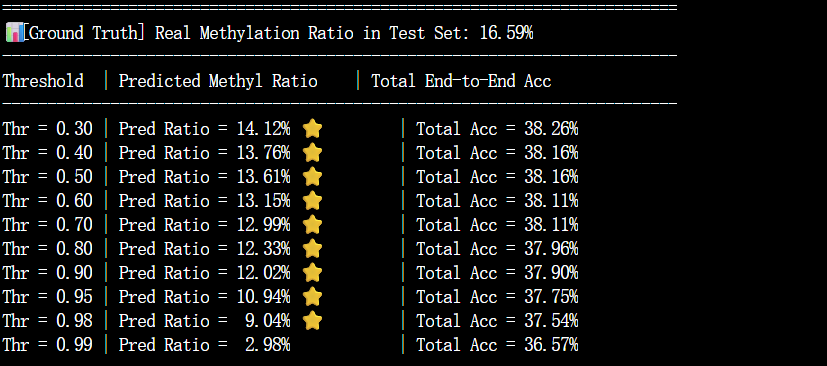
\includegraphics[width=0.94\textwidth]{supplementary/historical_padding_e2e_table.png}
  \caption{历史端到端阈值截图。该次运行的有效数组长度为 1947，其中 442 个为 padding，故比例不能用于论文。原始图片仅用于审计留档。}
  \label{fig:old-e2e}
\end{figure}

第二张截图可被另一种 batch 切分精确重构：有效数组长度为 $1505+386=1891$，正类仍是 323，padding 被当作阴性后阴性总数变成 1568。阈值 0.6 时混淆矩阵为 $TP=90$、$FP=38$、$TN=1530$、$FN=233$，从而得到截图中的 Accuracy 85.67\%、Precision 70.31\%、Recall 27.86\% 和 F1 39.91\%。若模型全部预测阴性，Accuracy 仍为
\begin{equation}
\frac{1568}{1891}=82.9191\%,
\end{equation}
正好对应截图在阈值 0.95--0.99 的 82.92\%。这说明结果会随 batch size 改变，而不是模型本身改变。

\begin{figure}[H]
  \centering
  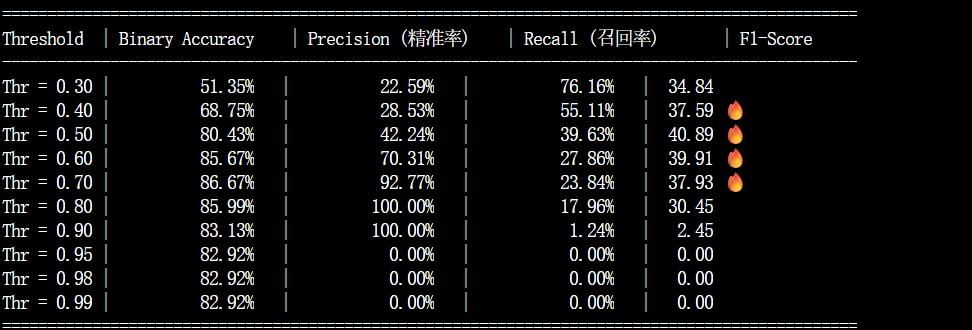
\includegraphics[width=0.94\textwidth]{supplementary/historical_padding_binary_table.png}
  \caption{历史二分类阈值截图。该次运行多计入 386 个 padding 阴性；所有显示值均可由错误混淆矩阵精确重构。}
  \label{fig:old-binary}
\end{figure}

根因是旧评价路径先按 padded batch 形状建立零初始化数组，再用不能排除这些有限零值的条件进入统计。padding 既没有真实残基，也没有合法甲基化标签，必须由真实长度/显式 mask 删除。附带的 \path{data/historical_padding_batch16_reconstruction.csv} 与 \path{data/historical_padding_batch8_reconstruction.csv} 保存了每个截图阈值的精确重构计数。

\subsection{去 padding 后，Ser 真值修正仍然必要}

只移除 padding、但继续使用旧 323 阳性标签时，已知序列 AUC 为 0.956，端到端 AUC 为 0.835；阈值 0.6 下，前者 Accuracy/Precision/Recall/F1 为 90.30\%/96.83\%/56.66\%/71.48\%，后者为 85.12\%/89.60\%/34.67\%/50.00\%。这些数值虽然已不受 padding 影响，但仍把 62 个本应为天然 Ser 的位点当作甲基阳性。

\begin{table}[H]
\centering
\caption{同一原始检查点在不同评价真值下的单体结果。阈值均为严格 $p>0.6$；旧标签只用于敏感性比较。}
\label{tab:label-sensitivity}
\begin{tabular}{L{30mm}L{31mm}rrrrr}
\toprule
真值版本 & 输入条件 & AUC & Accuracy & Precision & Recall & F1 \\
\midrule
旧 323 阳性 & 已知序列 & 0.956 & 90.30\% & 96.83\% & 56.66\% & 71.48\% \\
旧 323 阳性 & 端到端 & 0.835 & 85.12\% & 89.60\% & 34.67\% & 50.00\% \\
Ser 修正 261 阳性 & 已知序列 & 0.900 & 86.18\% & 64.02\% & 46.36\% & 53.78\% \\
Ser 修正 261 阳性 & 端到端 & 0.908 & 89.10\% & 88.80\% & 42.53\% & 57.51\% \\
\bottomrule
\end{tabular}
\end{table}

Ser 子集揭示了修正的影响：74 个 Ser 位点中只有 12 个为阳性；已知序列头在阈值 0.6 时把 74 个全部判为阳性，得到 $TP=12$、$FP=62$、$TN=0$、$FN=0$。因此，旧标签会把这 62 个系统性假阳性错误奖励为真阳性。正文采用修正后的 261/1244 真值，既不隐藏模型在 Ser 上的缺陷，也不因错误标签虚增性能。

\subsection{规划截图是指标清单，不是已完成数据}

\begin{figure}[H]
  \centering
  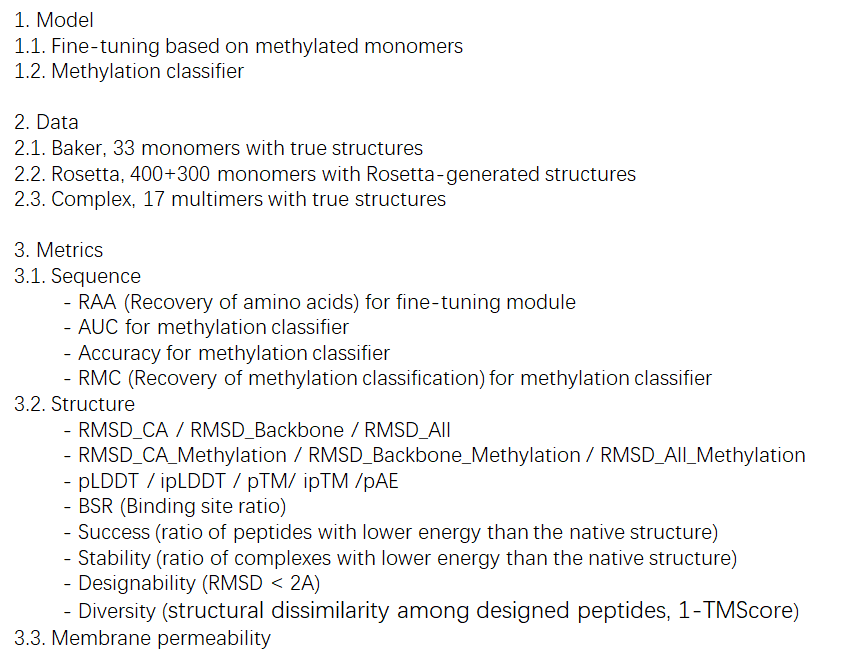
\includegraphics[width=0.92\textwidth]{supplementary/requested_metric_outline.png}
  \caption{尚哥提出的数据与指标规划截图。它定义了希望覆盖的项目，但不等于每项已经有原始结果；实际可用性逐项列于\cref{app:metric-matrix}。}
  \label{fig:metric-outline}
\end{figure}

截图中的 ``Baker, 33 monomers''、``Rosetta, 400+300 monomers'' 与冻结文件不一致。逐一审计 751 个原始 PDB 后，751/751 均含理论模型和 Rosetta 生成标记；406 个 \path{Me_} 对应 Rosetta-2023，345 个 \path{pdb_} 对应 Rosetta-2025。仓库、共享工作区与附件中均未找到可验证的 Baker 33 实验结构目录或清单。因此，本文采用“751 个 Rosetta 理论结构、600/151 划分”的可验证表述，不把规划截图冒充数据证据。

另有历史 V12 工作流的单体结构比较文件，但其检查点、结构队列和评价流程均不属于本文冻结的 V28 对象。为防止张冠李戴，本稿不移植其中任何数值；V28 单体结构指标仍明确标记为未计算。

\section{联合RMSD低于5~\AA{}的101条候选清单}
\label{app:pass-list}

表~\ref{tab:pass101}逐条列出六个非3AV复合物中同时满足全复合物CA RMSD
$<5~\angstrom$且最佳正向循环肽CA RMSD $<5~\angstrom$的101条候选。
这些候选均来自正文定义的476条保留设计，并沿用“一次全复合物叠合、完整末链
CA配对、最佳正向循环移位、不反向、不进行肽链二次拟合”的联合RMSD口径。
“类别”列进一步标出其中16条联合$<3~\angstrom$候选；其余85条位于
$[3,5)~\angstrom$类别。序列大小写保持原始输出，小写残基表示严格$p>0.6$
规则保存的预测甲基化标记，甲基化位点使用1基编号。

可复核的机器可读文件同时随稿提供：本表101条的完整记录位于
\path{data/Pass_LT5_101.csv}，其中16条联合$<3~\angstrom$候选另存于
\path{data/Pass_LT3_16.csv}；包含通过与未通过候选、各审计门控字段及两种
RMSD的完整476条分析表位于\path{data/Candidates_476.csv}。因此，本附录是便于
人工阅读的通过清单，完整统计复算应以476条CSV为准。

\begin{landscape}
\begingroup
\small
\setlength{\tabcolsep}{4pt}
\setlength\LTleft{0pt}
\setlength\LTright{0pt}
\captionof{table}{六个非 3AV 复合物中联合 RMSD 低于 5~\AA{} 的 101 条候选}
\label{tab:pass101}
\begin{longtable}{C{10mm} C{18mm} L{48mm} L{36mm} C{27mm} C{30mm} C{24mm}}
  \toprule
  编号 & 靶点 & 设计序列（小写为甲基化） & 甲基化位点 &
  \makecell{全复合物CA\\RMSD（\AA）} &
  \makecell{循环肽CA\\RMSD（\AA）} & 类别 \\
  \midrule
  \endfirsthead

  \multicolumn{7}{l}{\footnotesize 表~\ref{tab:pass101}（续）}\\
  \toprule
  编号 & 靶点 & 设计序列（小写为甲基化） & 甲基化位点 &
  \makecell{全复合物CA\\RMSD（\AA）} &
  \makecell{循环肽CA\\RMSD（\AA）} & 类别 \\
  \midrule
  \endhead

  \midrule
  \multicolumn{7}{r}{\footnotesize 续下页}\\
  \endfoot

  \bottomrule
  \endlastfoot

  1 & 1SFI & \seq{RCCrGNCGQCQFGG} & 4 & 0.536 & 2.818 & $<3$ \\
2 & 1SFI & \seq{RCGrGcCrQGcNGG} & 4,6,8,11 & 0.562 & 3.693 & $3\text{--}<5$ \\
3 & 1SFI & \seq{RCGrCQNGQCrNGG} & 4,11 & 1.120 & 3.840 & $3\text{--}<5$ \\
4 & 1SFI & \seq{RrGrGrCGQCQFMQ} & 2,4,6 & 1.483 & 3.859 & $3\text{--}<5$ \\
5 & 1SFI & \seq{CCGrGrCrQGrGGR} & 4,6,8,11 & 0.572 & 3.967 & $3\text{--}<5$ \\
6 & 1SFI & \seq{RCGrQQCrKGcQMC} & 4,8,11 & 0.817 & 4.217 & $3\text{--}<5$ \\
7 & 1SFI & \seq{RCGrGQCrKGrNGC} & 4,8,11 & 0.242 & 4.252 & $3\text{--}<5$ \\
8 & 1SFI & \seq{RrrrGQCrQCNRDG} & 2,3,4,8 & 1.805 & 4.276 & $3\text{--}<5$ \\
9 & 1SFI & \seq{RQYrGKGrQGrRMG} & 4,8,11 & 0.221 & 4.414 & $3\text{--}<5$ \\
10 & 1SFI & \seq{RGGrCcCGGGNQMG} & 4,6 & 1.068 & 4.468 & $3\text{--}<5$ \\
11 & 1SFI & \seq{RCHrCNGCQCrQGC} & 4,11 & 0.576 & 4.523 & $3\text{--}<5$ \\
12 & 1SFI & \seq{RrGcCrCrKGKFDG} & 2,4,6,8 & 0.632 & 4.532 & $3\text{--}<5$ \\
13 & 1SFI & \seq{RCGrGQCrKGrQDG} & 4,8,11 & 0.563 & 4.612 & $3\text{--}<5$ \\
14 & 1SFI & \seq{RCGrGrCrQCrQMC} & 4,6,8,11 & 0.970 & 4.626 & $3\text{--}<5$ \\
15 & 1SFI & \seq{CCrrrGCrKCNNNG} & 3,4,5,8 & 0.219 & 4.753 & $3\text{--}<5$ \\
16 & 1SFI & \seq{RrGrGrCGQCcQMG} & 2,4,6,11 & 1.854 & 4.756 & $3\text{--}<5$ \\
17 & 1SFI & \seq{RCrrrNNGGCrQGG} & 3,4,5,11 & 0.467 & 4.763 & $3\text{--}<5$ \\
18 & 1SFI & \seq{CCYrCrCrKGrFDG} & 4,6,8,11 & 0.228 & 4.776 & $3\text{--}<5$ \\
19 & 1SFI & \seq{RCGQGQCrQCrRDG} & 8,11 & 0.561 & 4.918 & $3\text{--}<5$ \\
20 & 3P8F & \seq{CrrrGrQGKGrRGC} & 2,3,4,6,11 & 0.300 & 2.075 & $<3$ \\
21 & 3P8F & \seq{GrGrGcCCQGrCMR} & 2,4,6,11 & 0.995 & 2.713 & $<3$ \\
22 & 3P8F & \seq{GrrrCrCGQCrNMG} & 2,3,4,6,11 & 0.559 & 3.255 & $3\text{--}<5$ \\
23 & 3P8F & \seq{CrhQrGCRrCQCGN} & 2,3,5,9 & 0.277 & 3.523 & $3\text{--}<5$ \\
24 & 3P8F & \seq{CCGrrQCRQCrCRC} & 4,5,11 & 0.311 & 3.807 & $3\text{--}<5$ \\
25 & 3P8F & \seq{RCrrGKCGQGrGCG} & 3,4,11 & 1.063 & 3.847 & $3\text{--}<5$ \\
26 & 3P8F & \seq{RrrrrGCGQCrCGG} & 2,3,4,5,11 & 1.556 & 3.854 & $3\text{--}<5$ \\
27 & 3P8F & \seq{RCrrrrGGQCrCMN} & 3,4,5,6,11 & 0.648 & 3.862 & $3\text{--}<5$ \\
28 & 3P8F & \seq{RrKrGQCRQGcrRG} & 2,4,11,12 & 0.522 & 3.965 & $3\text{--}<5$ \\
29 & 3P8F & \seq{RrrrGNCCKCrCDG} & 2,3,4,11 & 1.599 & 4.081 & $3\text{--}<5$ \\
30 & 3P8F & \seq{RrrrGNCGKCrRRG} & 2,3,4,11 & 1.708 & 4.303 & $3\text{--}<5$ \\
31 & 3P8F & \seq{QrrrGQCGFCrQMG} & 2,3,4,11 & 1.456 & 4.356 & $3\text{--}<5$ \\
32 & 3P8F & \seq{RrhrCKCCrCrCMG} & 2,3,4,9,11 & 0.291 & 4.363 & $3\text{--}<5$ \\
33 & 3P8F & \seq{RCGrGGCRQCrRCC} & 4,11 & 1.002 & 4.449 & $3\text{--}<5$ \\
34 & 3P8F & \seq{RrrrGKCGQGrCMG} & 2,3,4,11 & 1.105 & 4.496 & $3\text{--}<5$ \\
35 & 3P8F & \seq{GrGrGNCRQCrFMG} & 2,4,11 & 0.405 & 4.668 & $3\text{--}<5$ \\
36 & 3P8F & \seq{RCrrrNCGQCrQDG} & 3,4,5,11 & 1.323 & 4.757 & $3\text{--}<5$ \\
37 & 3P8F & \seq{CrrrGQCGQCrrMG} & 2,3,4,11,12 & 1.266 & 4.791 & $3\text{--}<5$ \\
38 & 3P8F & \seq{RrrrQNCGQGrCMG} & 2,3,4,11 & 0.289 & 4.883 & $3\text{--}<5$ \\
39 & 3P8F & \seq{RCGrGGCGNCrCGG} & 4,11 & 1.048 & 4.921 & $3\text{--}<5$ \\
40 & 3WNE & \seq{GrKWNC} & 2 & 0.933 & 1.459 & $<3$ \\
41 & 3WNE & \seq{GrGKFG} & 2 & 0.904 & 2.915 & $<3$ \\
42 & 3WNE & \seq{GrGWQG} & 2 & 0.904 & 2.946 & $<3$ \\
43 & 3WNE & \seq{GrGKGG} & 2 & 0.912 & 3.407 & $3\text{--}<5$ \\
44 & 3WNE & \seq{GrNWRG} & 2 & 1.041 & 3.868 & $3\text{--}<5$ \\
45 & 3ZGC & \seq{rEGGQNR} & 1 & 0.973 & 2.076 & $<3$ \\
46 & 3ZGC & \seq{NrGGGQR} & 2 & 1.488 & 2.231 & $<3$ \\
47 & 3ZGC & \seq{rrGGLGR} & 1,2 & 0.988 & 3.103 & $3\text{--}<5$ \\
48 & 3ZGC & \seq{rrNGGGR} & 1,2 & 0.968 & 3.233 & $3\text{--}<5$ \\
49 & 3ZGC & \seq{cGGGQDR} & 1 & 1.589 & 3.516 & $3\text{--}<5$ \\
50 & 3ZGC & \seq{rGcGQGR} & 1,3 & 1.600 & 3.759 & $3\text{--}<5$ \\
51 & 3ZGC & \seq{EcGQGMR} & 2 & 1.194 & 3.769 & $3\text{--}<5$ \\
52 & 3ZGC & \seq{cCGGGNR} & 1 & 1.476 & 4.100 & $3\text{--}<5$ \\
53 & 3ZGC & \seq{rGGGNLR} & 1 & 2.226 & 4.123 & $3\text{--}<5$ \\
54 & 3ZGC & \seq{rrGGQDR} & 1,2 & 0.919 & 4.129 & $3\text{--}<5$ \\
55 & 3ZGC & \seq{rGGGQGR} & 1 & 2.535 & 4.262 & $3\text{--}<5$ \\
56 & 3ZGC & \seq{GrGGNQR} & 2 & 1.847 & 4.281 & $3\text{--}<5$ \\
57 & 3ZGC & \seq{rGGGGMR} & 1 & 2.742 & 4.367 & $3\text{--}<5$ \\
58 & 3ZGC & \seq{cGGGQQR} & 1 & 2.443 & 4.370 & $3\text{--}<5$ \\
59 & 3ZGC & \seq{rGGGQFR} & 1 & 2.337 & 4.454 & $3\text{--}<5$ \\
60 & 3ZGC & \seq{cGGGGDR} & 1 & 2.344 & 4.456 & $3\text{--}<5$ \\
61 & 3ZGC & \seq{cGGGQGR} & 1 & 2.284 & 4.469 & $3\text{--}<5$ \\
62 & 3ZGC & \seq{rGGGGDR} & 1 & 1.651 & 4.618 & $3\text{--}<5$ \\
63 & 3ZGC & \seq{cGGGGLR} & 1 & 2.967 & 4.651 & $3\text{--}<5$ \\
64 & 3ZGC & \seq{rGDGGGR} & 1 & 1.801 & 4.686 & $3\text{--}<5$ \\
65 & 3ZGC & \seq{rGGGQCR} & 1 & 2.553 & 4.750 & $3\text{--}<5$ \\
66 & 3ZGC & \seq{cGGGKGR} & 1 & 2.274 & 4.767 & $3\text{--}<5$ \\
67 & 3ZGC & \seq{rGGGQMR} & 1 & 2.744 & 4.898 & $3\text{--}<5$ \\
68 & 4K1E & \seq{rcrrrQCrQGNCDR} & 1,2,3,4,5,8 & 0.900 & 1.916 & $<3$ \\
69 & 4K1E & \seq{rcrrCrCrFGQCMR} & 1,2,3,4,6,8 & 0.637 & 2.157 & $<3$ \\
70 & 4K1E & \seq{rcCrGrQrNGERLR} & 1,2,4,6,8 & 0.821 & 2.330 & $<3$ \\
71 & 4K1E & \seq{rcCrrrQrQCQCDR} & 1,2,4,5,6,8 & 0.694 & 2.596 & $<3$ \\
72 & 4K1E & \seq{rcrrGrCrQGhCLR} & 1,2,3,4,6,8,11 & 0.680 & 2.801 & $<3$ \\
73 & 4K1E & \seq{CcCrrrRrQCrRLC} & 2,4,5,6,8,11 & 0.659 & 2.960 & $<3$ \\
74 & 4K1E & \seq{CcGrCQCrEGFRDR} & 2,4,8 & 0.920 & 3.273 & $3\text{--}<5$ \\
75 & 4K1E & \seq{rcrrrcCrFGQCDR} & 1,2,3,4,5,6,8 & 0.676 & 3.338 & $3\text{--}<5$ \\
76 & 4K1E & \seq{rcrrCrRrQGcCWR} & 1,2,3,4,6,8,11 & 0.644 & 3.368 & $3\text{--}<5$ \\
77 & 4K1E & \seq{rcQrrrGrQCQCDR} & 1,2,4,5,6,8 & 0.646 & 3.511 & $3\text{--}<5$ \\
78 & 4K1E & \seq{rrGrGrCrFCLRGR} & 1,2,4,6,8 & 1.221 & 3.661 & $3\text{--}<5$ \\
79 & 4K1E & \seq{rrrrGNQrQGQCMC} & 1,2,3,4,8 & 0.690 & 3.672 & $3\text{--}<5$ \\
80 & 4K1E & \seq{rcrrCrQrrCQCMR} & 1,2,3,4,6,8,9 & 0.665 & 3.714 & $3\text{--}<5$ \\
81 & 4K1E & \seq{rrrrCrCrRCQCMR} & 1,2,3,4,6,8 & 0.697 & 3.818 & $3\text{--}<5$ \\
82 & 4K1E & \seq{rcrrrrCrQCQRDR} & 1,2,3,4,5,6,8 & 1.432 & 3.950 & $3\text{--}<5$ \\
83 & 4K1E & \seq{rcCrrGQrrCQrDR} & 1,2,4,5,8,9,12 & 0.691 & 4.045 & $3\text{--}<5$ \\
84 & 4K1E & \seq{rcNrrrCrQGQCDR} & 1,2,4,5,6,8 & 1.627 & 4.420 & $3\text{--}<5$ \\
85 & 4K1E & \seq{rcKrrrCrCCLNWR} & 1,2,4,5,6,8 & 0.679 & 4.464 & $3\text{--}<5$ \\
86 & 4K1E & \seq{rcCrGrCrQCNCDR} & 1,2,4,6,8 & 0.761 & 4.526 & $3\text{--}<5$ \\
87 & 4K1E & \seq{rQrrGrCrKCNCDR} & 1,3,4,6,8 & 1.878 & 4.594 & $3\text{--}<5$ \\
88 & 4K1E & \seq{rQCrGrCrQGFrDR} & 1,4,6,8,12 & 0.774 & 4.694 & $3\text{--}<5$ \\
89 & 4K1E & \seq{rcGrCrCrQCQCMR} & 1,2,4,6,8 & 0.763 & 4.751 & $3\text{--}<5$ \\
90 & 4K1E & \seq{rcrrGrCrFCQCGC} & 1,2,3,4,6,8 & 1.156 & 4.927 & $3\text{--}<5$ \\
91 & 4K1E & \seq{rcCrCrNrQGECDR} & 1,2,4,6,8 & 1.094 & 4.970 & $3\text{--}<5$ \\
92 & 4KEL & \seq{RcrrGNCrQGFCDR} & 2,3,4,8 & 0.654 & 2.379 & $<3$ \\
93 & 4KEL & \seq{CcCrCNQrFGQRDR} & 2,4,8 & 1.188 & 2.477 & $<3$ \\
94 & 4KEL & \seq{RcrrGrCWFCQRGR} & 2,3,4,6 & 0.988 & 3.421 & $3\text{--}<5$ \\
95 & 4KEL & \seq{RrGrrrRrQGrRDR} & 2,4,5,6,8,11 & 0.695 & 4.174 & $3\text{--}<5$ \\
96 & 4KEL & \seq{RcrrrQCrQGrCLR} & 2,3,4,5,8,11 & 0.657 & 4.267 & $3\text{--}<5$ \\
97 & 4KEL & \seq{RrrrCQCQrGLCGR} & 2,3,4,9 & 0.666 & 4.367 & $3\text{--}<5$ \\
98 & 4KEL & \seq{RcrKGrNrQGQCDR} & 2,3,6,8 & 1.426 & 4.595 & $3\text{--}<5$ \\
99 & 4KEL & \seq{RcCrGQNrQGQCGR} & 2,4,8 & 1.061 & 4.715 & $3\text{--}<5$ \\
100 & 4KEL & \seq{CGrrGrCrQGrCGR} & 3,4,6,8,11 & 1.545 & 4.871 & $3\text{--}<5$ \\
101 & 4KEL & \seq{RcrrrrCrFCrRDR} & 2,3,4,5,6,8,11 & 0.679 & 4.984 & $3\text{--}<5$ \\

\end{longtable}
\endgroup
\end{landscape}

\section{可复现性、文件索引与使用方法}
\label{app:reproducibility}

\subsection{本稿如何生成}

本稿采用“复用已生成文件、不重新跑上游模型”的冻结策略。素材脚本只完成确定性的文件复制、CSV 导出、历史截图计数重构和汇总图生成；不会载入检查点，也不会调用结构预测、通透性模型或 PyRosetta。脚本入口见 \path{scripts/prepare_paper_assets.py}。论文中的每项数值必须回到 \path{data/}、\path{supplementary/} 或源清单。

\begin{table}[H]
\centering
\caption{交付目录索引。}
\label{tab:file-index}
\begin{tabularx}{\textwidth}{L{39mm}Y}
\toprule
路径 & 内容 \\
\midrule
\path{main.tex}, \path{main.pdf} & 中文 LaTeX 源稿与已编译 PDF \\
\path{sections/} & 正文和附录各章节 \\
\path{figures/} & 6 组论文图，提供 PDF/PNG/SVG \\
\path{data/} & 主表 CSV、476 条审计、101/16 条通过名单及探索性结果 \\
\path{tables/} & 101 条联合 RMSD $<5$~\AA{} 候选的 LaTeX 表格行 \\
\path{supplementary/} & 两个 Excel 工作簿、历史阈值截图与指标提纲截图 \\
\path{fonts/} & 中文子集字体、原版权声明、修改记录及 SIL OFL 1.1 许可证 \\
\path{SOURCE_MANIFEST.json} & 上游关键文件路径、字节数和 SHA-256 \\
\path{scripts/} & 素材整理脚本与751个 PDB 来源审计脚本 \\
\path{requirements-assets.txt} & 更新论文素材所需的固定 Python 依赖版本 \\
\path{build.ps1}, \path{build.sh} & Windows PowerShell 与 Linux/macOS 构建入口 \\
\bottomrule
\end{tabularx}
\end{table}

\subsection{冻结标识与检查项}

\begin{itemize}
  \item 模型文件：\path{frankenstein_v28.pt}；
  \item 模型 SHA-256（完整值）：\\
  \texttt{bab7b8a010114fc52c749fab1914d9d8}\\
  \texttt{ae561ddca45d6d7a0fbec3f9f5ac5b2e}；
  \item 仓库：\path{DCarchimonde/proteinmpnn-clean-v28}；
  \item 基线提交：\texttt{c9718e2a\allowbreak{}433a51f1\allowbreak{}87606676\allowbreak{}dfedd11e\allowbreak{}eb6fc8a5}；
  \item 论文分支：\path{paper/task1-original-v28-cn-2026-08-21}；
  \item 单体主分母：151 条、1505 位点、261 阳性、1244 阴性；
  \item 六复合物主分母：544 条原始，476 条甲基保留，476 条 RMSD 成功匹配；
  \item 17 靶点 best85：85/85 结构映射；置信度 COMMENT 字段仅 37/85；
  \item 所有概率门均为严格 $>0.6$，所有 RMSD 门均为严格 $<d$；
  \item 101 条 $<5$~\AA 与 16 条 $<3$~\AA 名单均可由 \path{Candidates_476.csv} 重新筛选得到。
\end{itemize}

\subsection{本地编译}

仓库已经提交编译后的 \path{main.pdf}，仅阅读不需要安装 LaTeX。若要改稿重编译，在论文目录执行：

\begin{verbatim}
# Windows PowerShell
.\build.ps1

# Linux/macOS
bash build.sh
\end{verbatim}

构建脚本使用 XeLaTeX、BibTeX、XeLaTeX 两遍，以解析中文、目录、交叉引用与文献。中文正文使用仓库内随稿提供的子集字体，不依赖系统安装 \path{ctex} 或中文字体。若上游数据有意更新，应先运行 \texttt{python }\path{scripts/prepare_paper_assets.py}，随后重编译；维护者工作区中的上游文件不存在时，该脚本复用随稿的冻结副本。任何更新都应同时修改版本、日期与 \path{SOURCE_MANIFEST.json}。重新扫描751个原始 PDB 则需另行检出源清单中冻结的历史仓库提交。

\subsection{解释规则}

复核本稿时应始终保留以下边界：条件通过率不等于原始端到端产率；肽自拟合 RMSD 不等于结合姿态；B-factor/pLDDT 不等于能量；fixed-pose Rosetta 分数不等于结合自由能；oracle best-of-N 不等于盲生成性能；未计算和不可定义不等于零。这些规则也是后续 V8/V9 比较必须沿用的共同基线。


\clearpage
\bibliographystyle{unsrt}
\bibliography{references}

\end{document}
